\chapter{ Results \& Analysis } % Main chapter title

\label{Chapter4} % For referencing the chapter elsewhere, use \ref{Chapter1} 
 
\section{Justification of Working of Monitoring Box}

The System Architecture proposes a Box fitted with Gas pollutants measuring sensors comprises of (CO2, CO, PM) along with Temperature and Humidity. So we have tried to test that whether our sensors are able to catch the pollutants. So we designed an experiment with the by lighting a matchstick. A match sticks burned for around 15 seconds and we know that It produces gases like (CO2 and CO) during its burning. So we took a matchstick and tested with our made box and we have got some interesting results during the process. The Results are as follows:

\begin{figure}
\centering
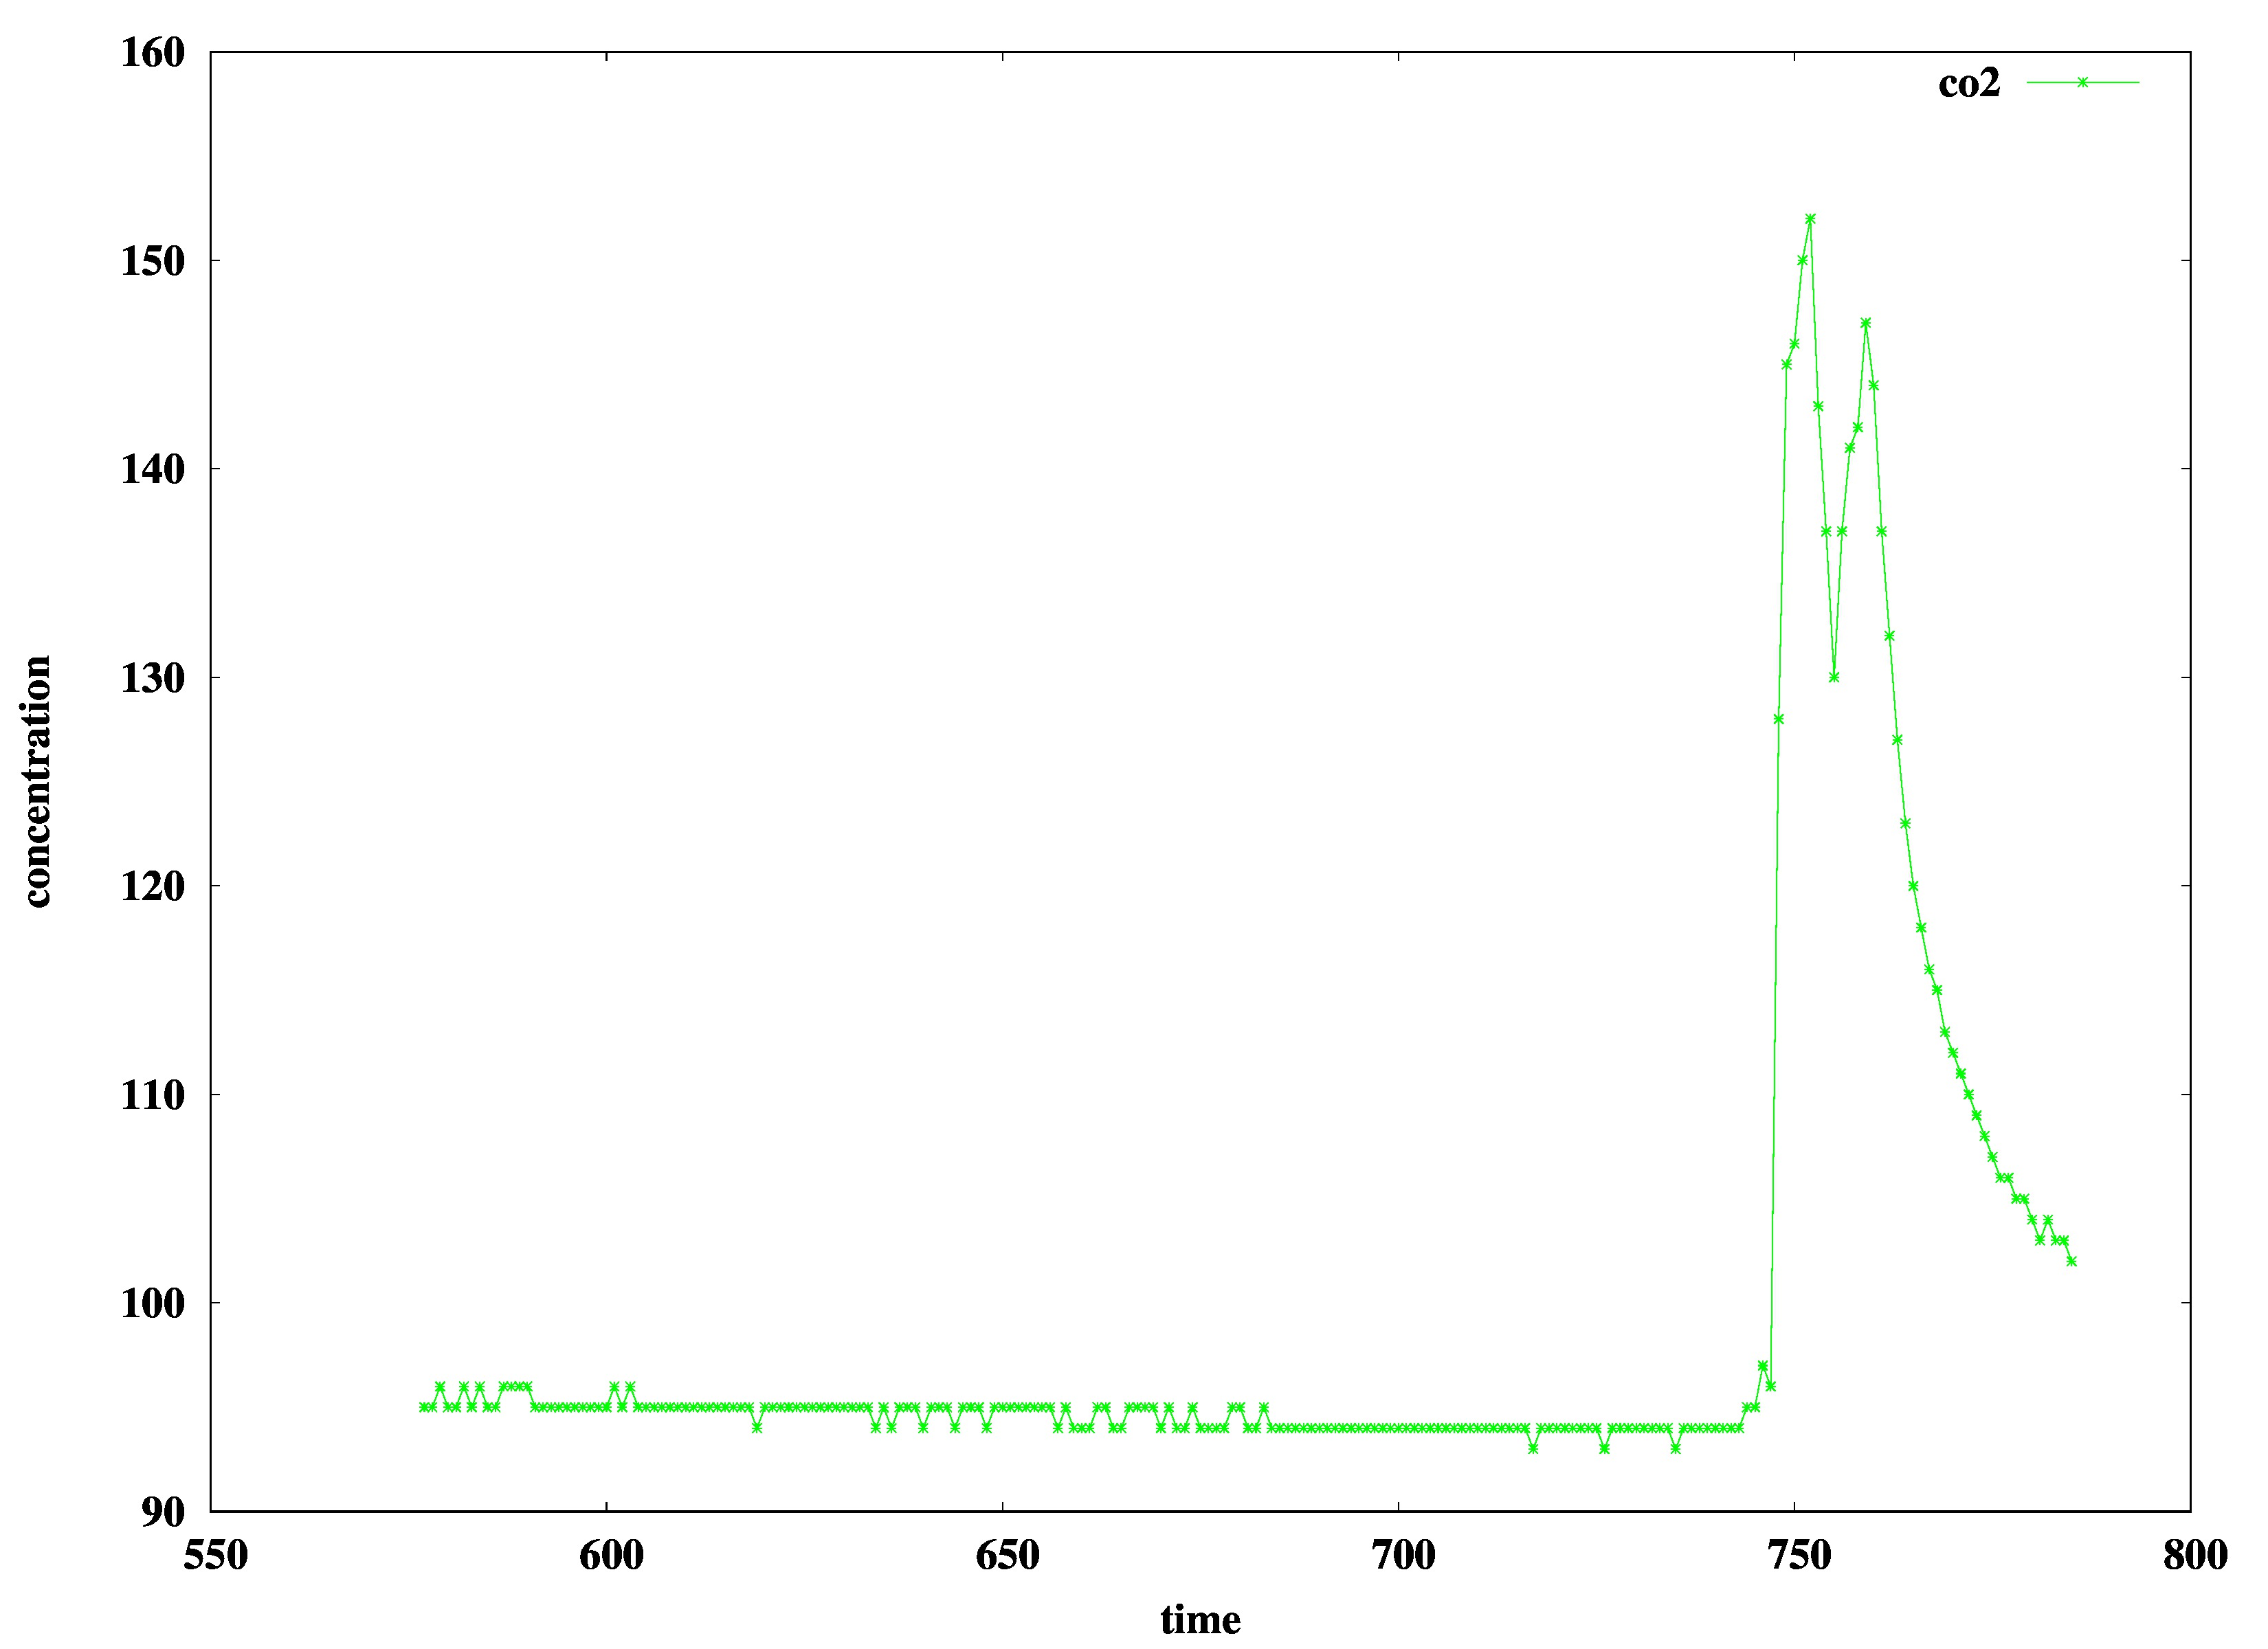
\includegraphics[width=0.9\textwidth]{./co2_match1}\\[0.1in]
\label{fig:$CO_2$ match testing}
\caption{$CO_2$ match testing(plot a)}
\end{figure}
\begin{figure}
\centering
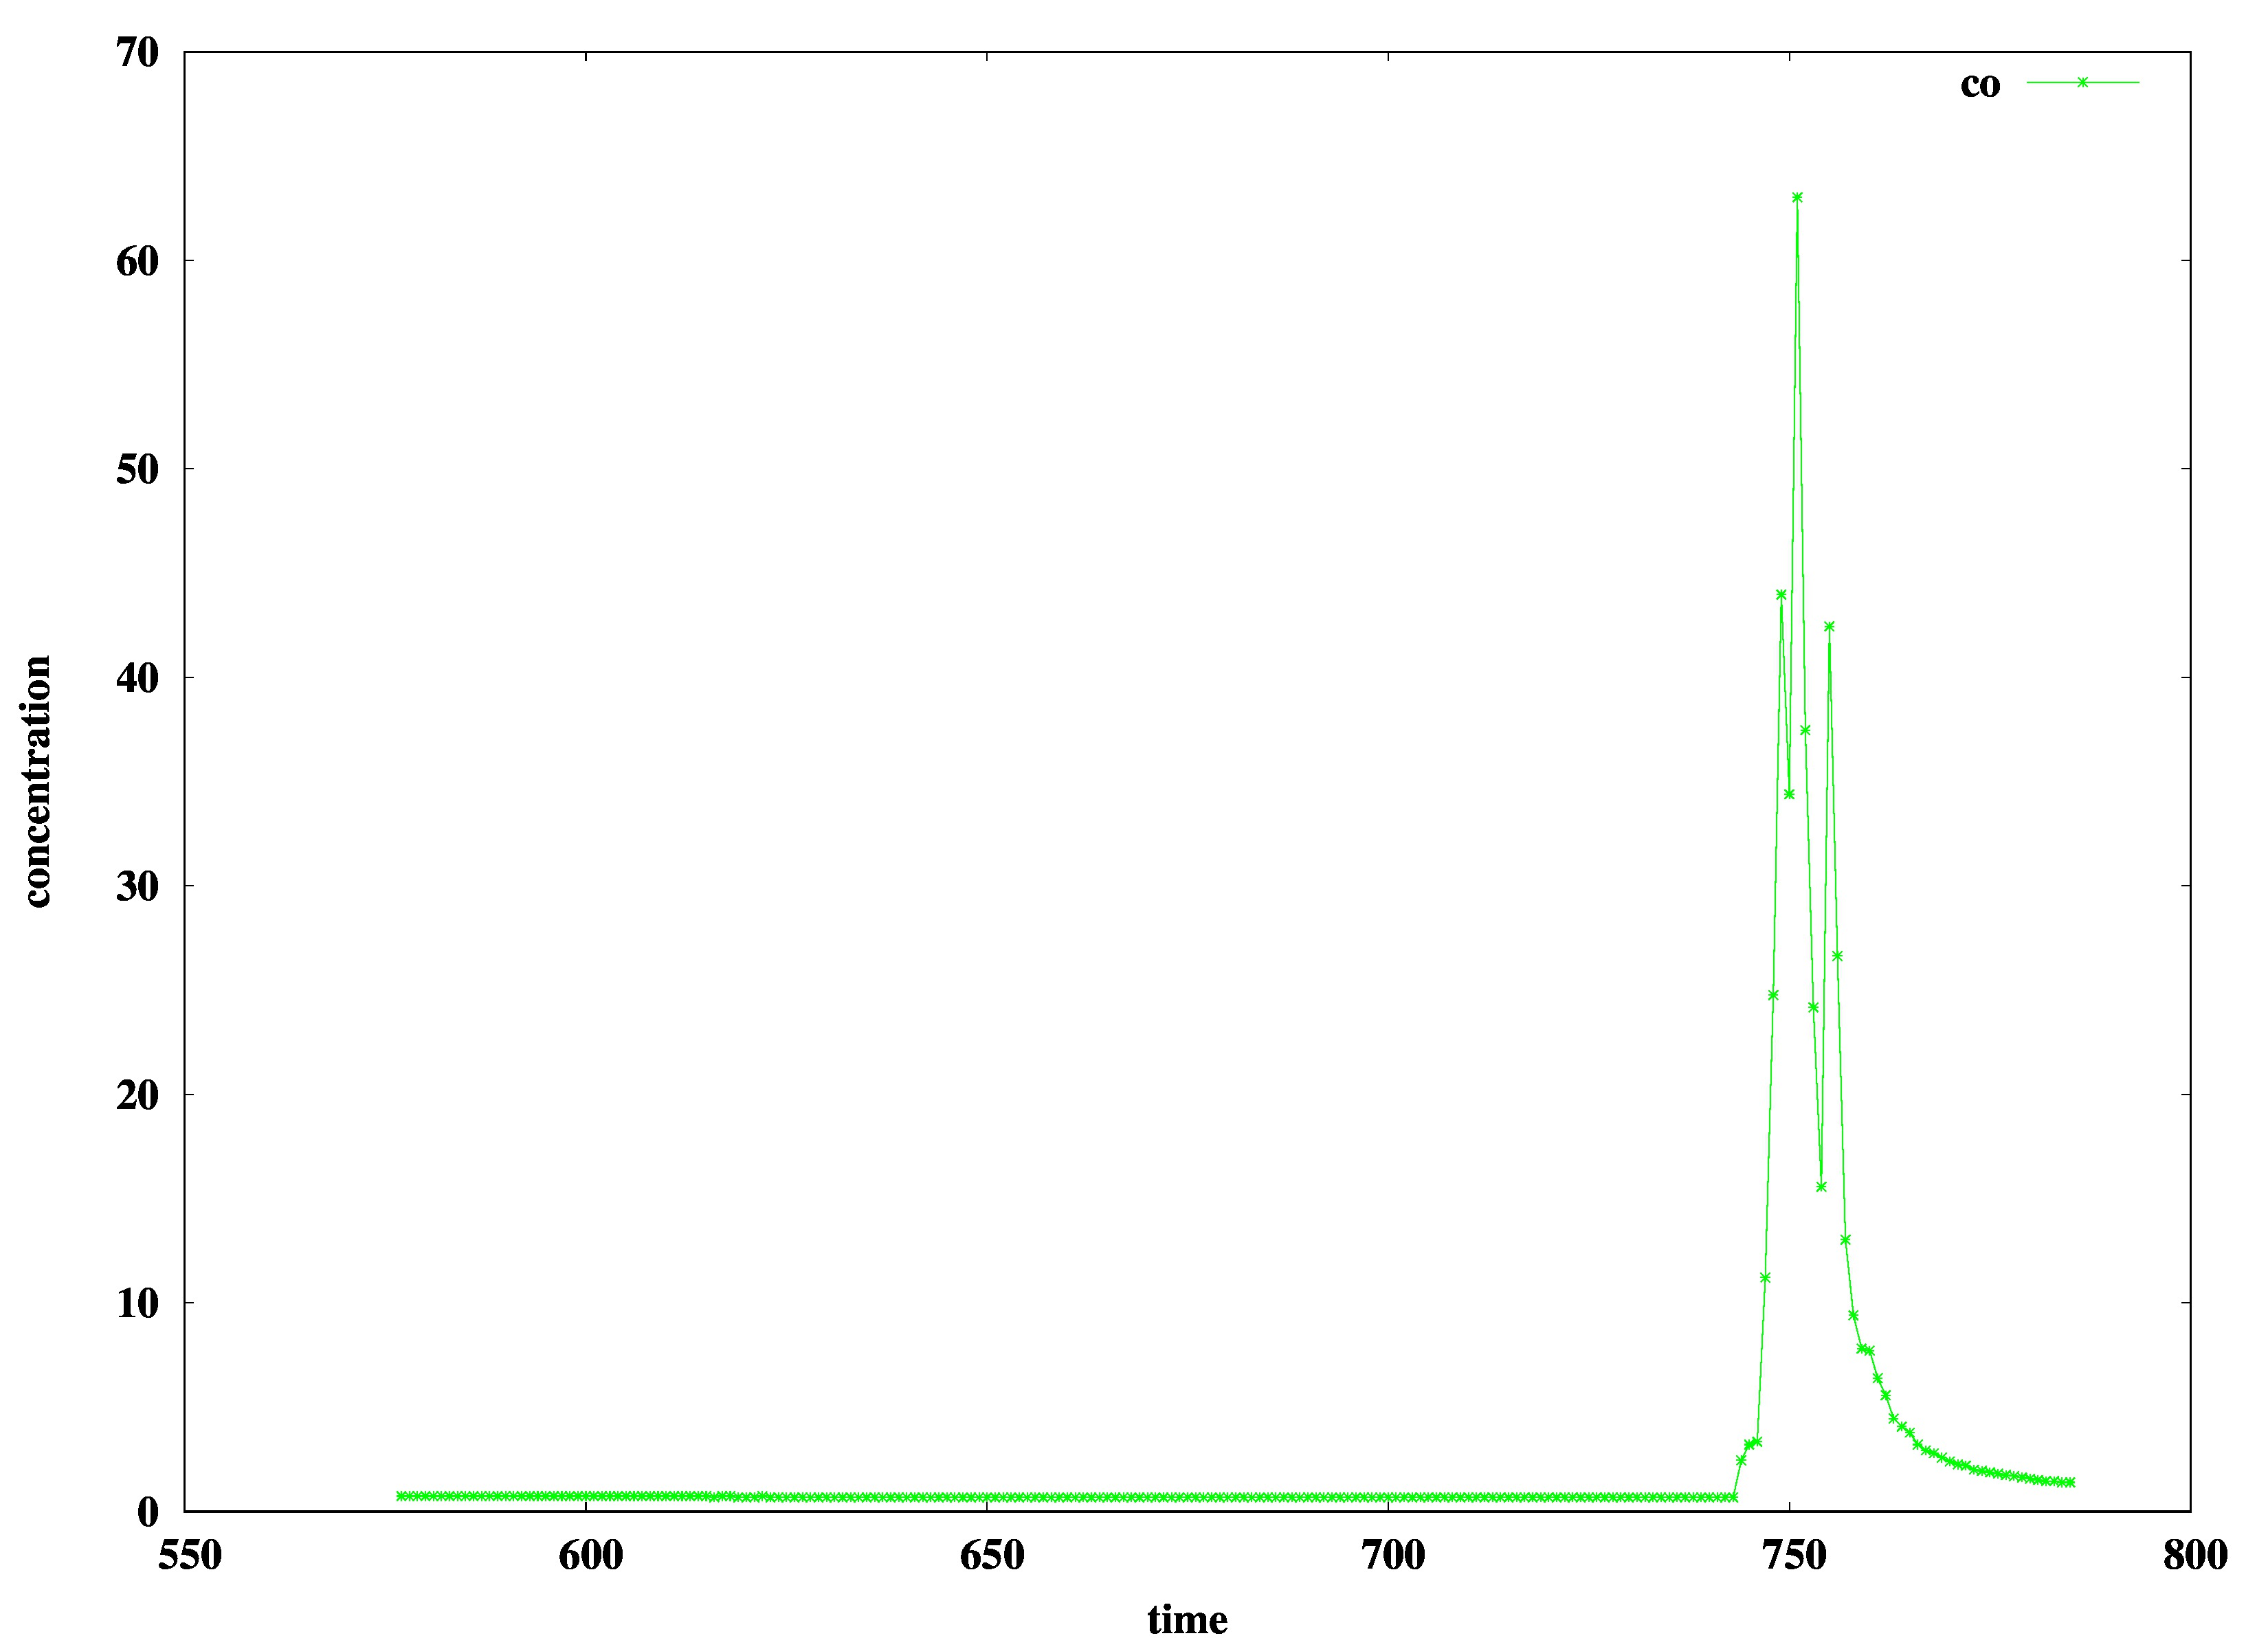
\includegraphics[width=0.9\textwidth]{./co_match1}\\[0.1in]
\label{CO match testing}
\caption{CO match testing(plot b)}
\end{figure}

Plot (a) shows the variation of $CO_2$ during the time period (note time axis is 2 data in a second) from (750 to around 780 count) we can see a significance rise in $CO_2$ pollutants to double of its initial reading (i.e 80 ppm to 150 ppm) during the tenure of matchstick burn.
\\
\\
Also Plot (b) which is the CO variation during the time frame showed a significant variation for the same.
\\
\\
This experiments proves that our box can catch significant variation on pollutants reading and also it is sensitive enough to catch variation over small time frame.

\section{Results for the Motivational Survey of our Project}

Today the whole world is suffering from the plague of pollution. Whole ecosystem has been affected adversely. Keeping ourselves in home, offices and indoor will not prevent us from getting affected by the contaminated air. To analyse the effects of pollutants in indoor environment, we have done some survey where it is seen that how badly some pollutants are affecting the classroom \& laboratory environment.
\\
\\
In the data collected from the students of a class we have studied some features of the classroom environment, (a) ratings of the class environment by students, (b) feel of suffocation in the environment, (c) duration of the class for which the data has been collected
\\
\\
We have done a survey for a classroom of 40 students and we have taken two cases in our survey, (a) feeling of suffocation, and (b) feeling of overall environment of the classroom. Fig. (1a) explains the observations from the data taken from the survey(b), it is seen that environment of the class has got only 10\% ratings as ’poor’, whereas it has got 90\% ratings as ’good’ for a class duration of 1 hour whereas in the same classroom for class duration of 2 hours, 40\% of the students rates the environment as poor. At the same time the suffocation has also been surveyed and result shown in Fig. (1b), which reports that, In the class of one-hour suffocation percentage is 25\% which is further increase to 62\% in the class of two hours. This can be understood easily from the Table 1
\begin{figure}
\centering
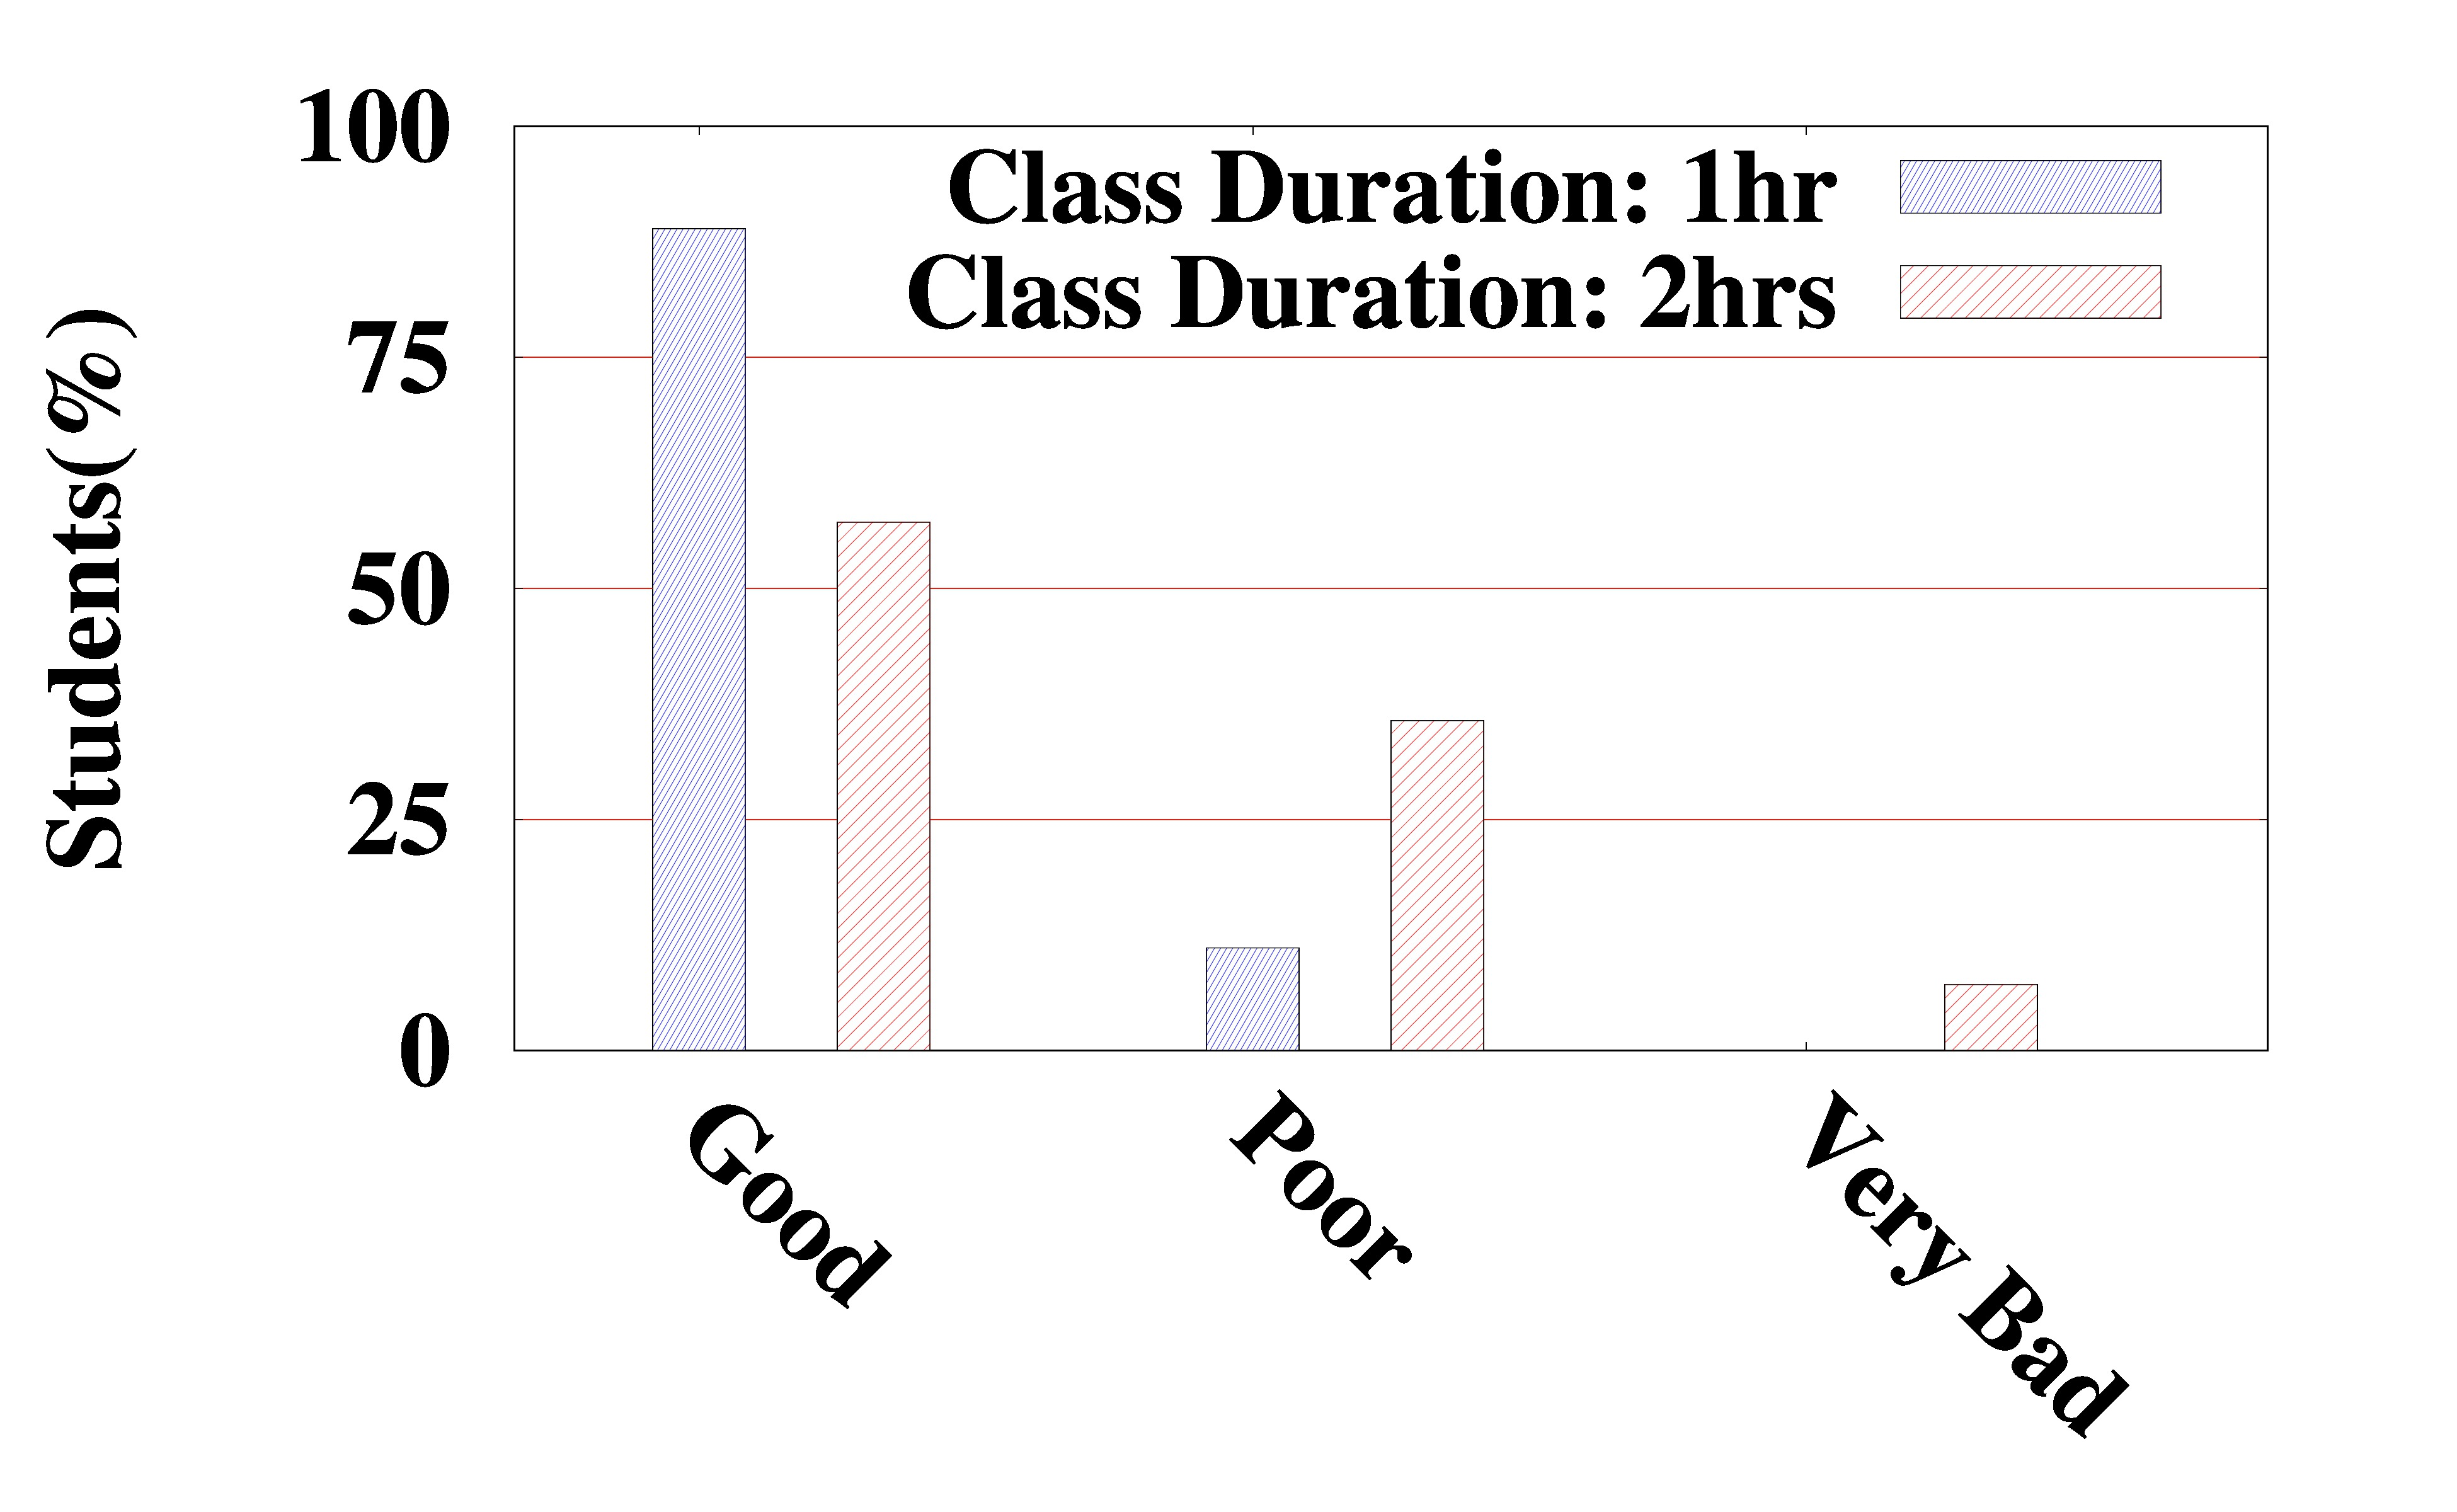
\includegraphics[width=1.0\textwidth]{./Ratings_1hr_2hrs}\\[0.1in]
\label{fig:Environment of class}
\caption{Environment of class}
\end{figure}
\begin{figure}
\centering
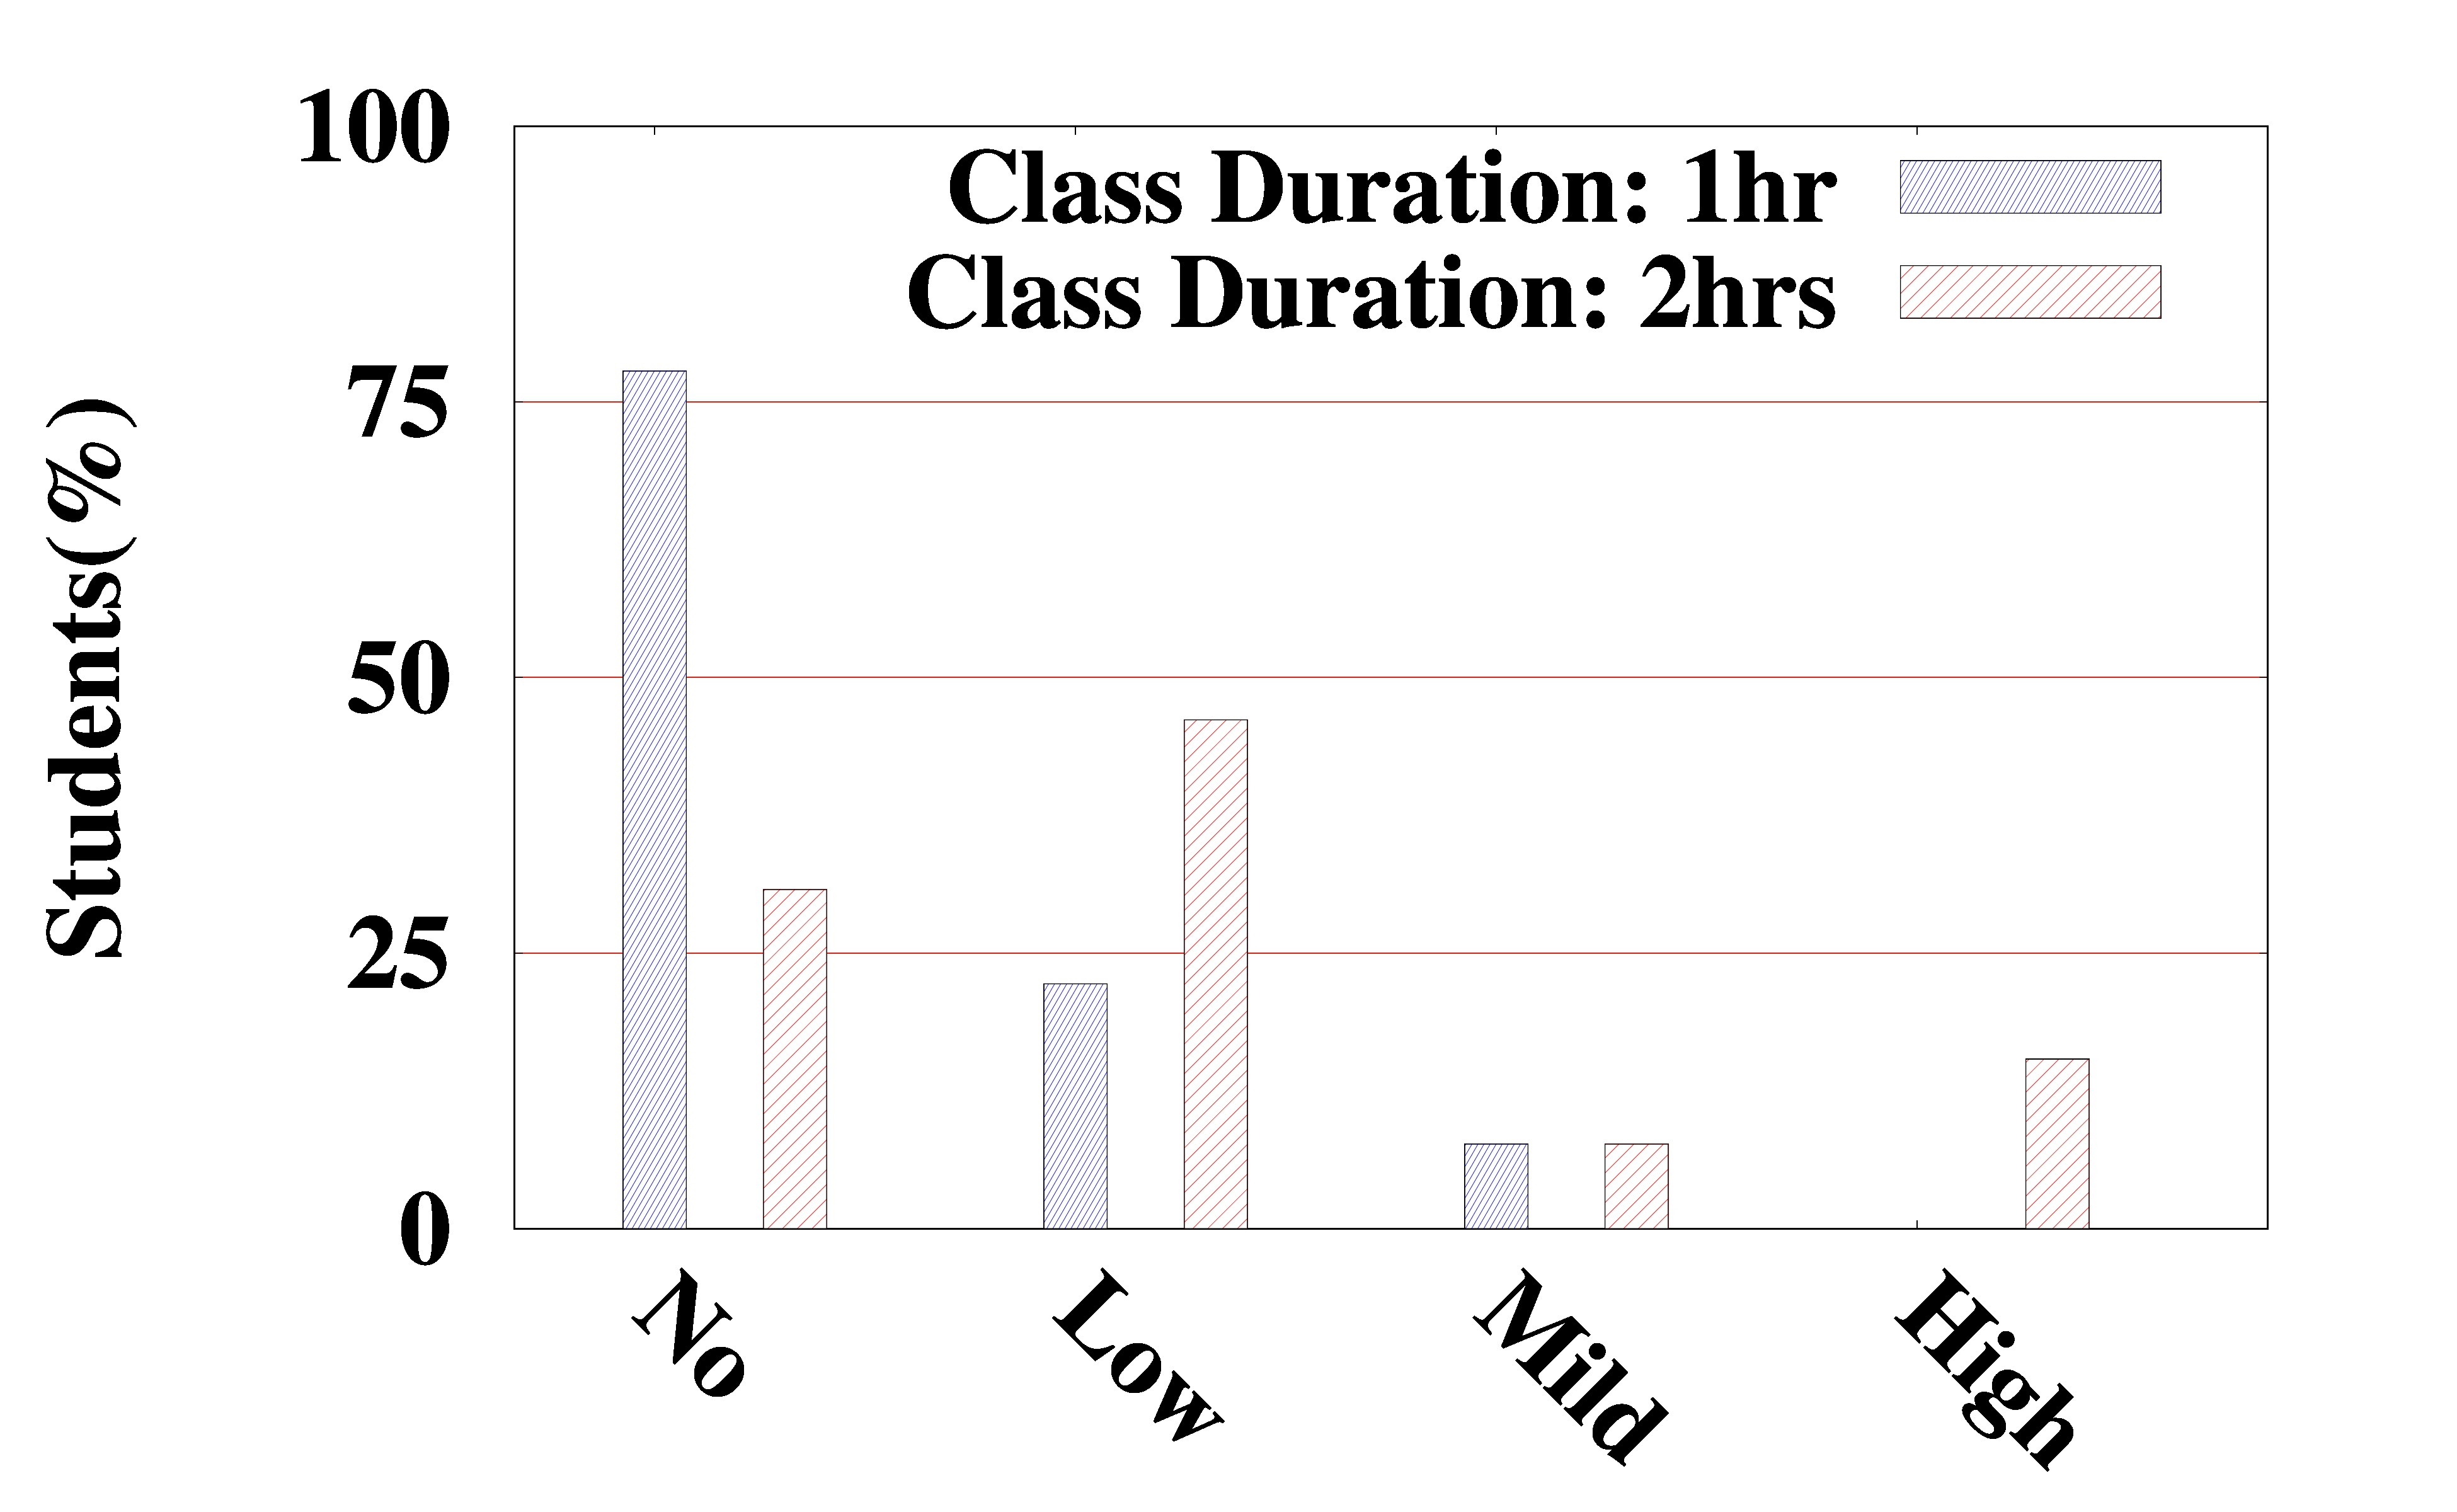
\includegraphics[width=1.0\textwidth]{./suffocation_1hr_2hrs}\\[0.1in]
\label{fig:feeling of suffocation}
\caption{feeling of suffocation}
\end{figure}

From the survey it is clear that the duration of a class is an important feature which infers some information as follow:
\begin{itemize}
	\item Most of the students feel good in the starting hour of the class.
	\item Most of the students start feeling suffocated if the class duration is long.
	\item Most of the students start feeling even more suffocated and irritation if the no. of students is more in the same class duration as mentioned in above point.
	\item Most of them rated the environment good at less no. of students and worst if the no. of students and duration of the classes increase.
\end{itemize}

\section{Experimental Setup}
After analysing the survey, we needed to find what is going wrong with the classes when the duration was getting longer so we designed an experiment to find out the variation of concentrations like (CO, CO2, PM 2.5, Temperature and Humidity) over time.
\\
\\
The Specifications of our environmental setup are as follows:
\\
\\
\begin{enumerate}
	\item \textbf{Classroom}: The classroom with dimension (8 X 7 X 2.54) m3 having one door with 3 windows and 6 fans as ventilation and air circulation.
	\item \textbf{Device Placement}: The device was placed 110 cm away from the window at a height of 60 cm.
	\item \textbf{Class Scenario}: The class was analysed with different strengths of 30, 40 and 60 students. Also Empty classroom data was also taken. 
\end{enumerate}

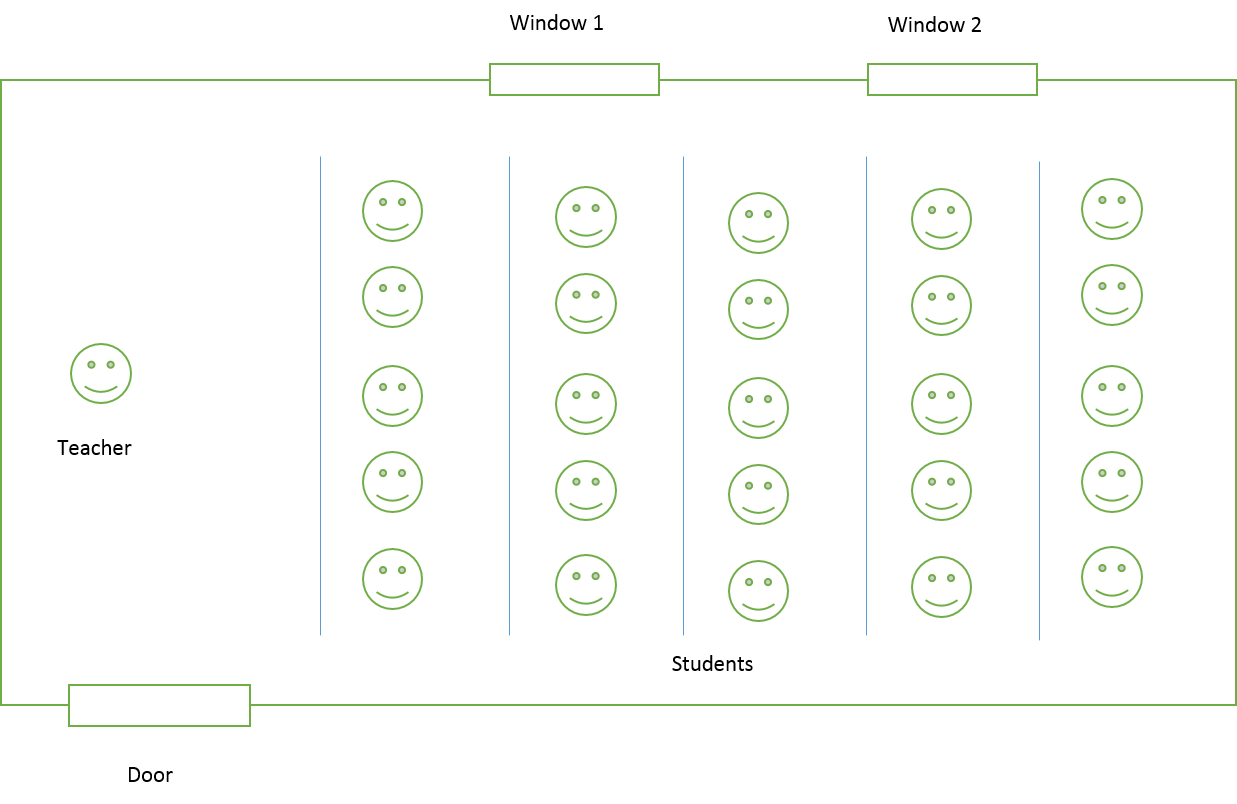
\includegraphics[width=1.0\textwidth]{./class}\\[0.1in]
\label{Classroom monitoring}

\section{Experimental Results}
The Datasets for pollutants along with temperature and humidity for the classrooms were taken for an interval of about two hours which is the standard duration of our classes. After Analysis of the data we have got significant results and some statistical evidence for justifying the scenario.
\begin{figure}
\centering
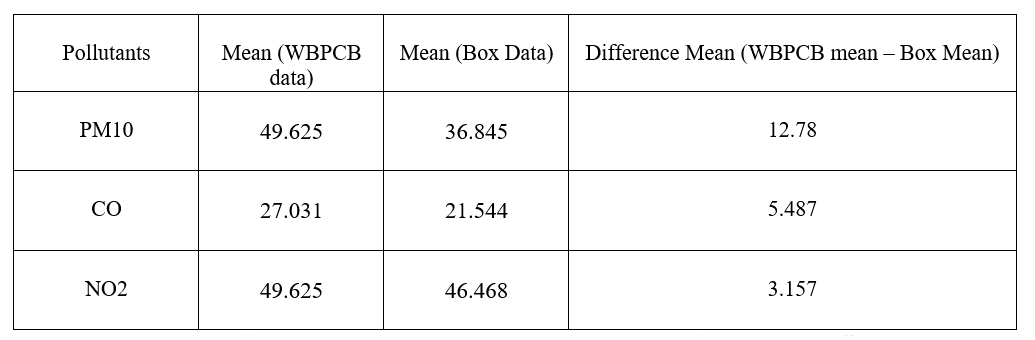
\includegraphics[width=1.0\textwidth]{./table}\\[0.1in]
\label{fig:Experimental result}
\caption{Experiment result}
\end{figure}


\begin{figure}
	\centering
	\hfill
	\centering
	\subfigure[Impact of $CO_2$]{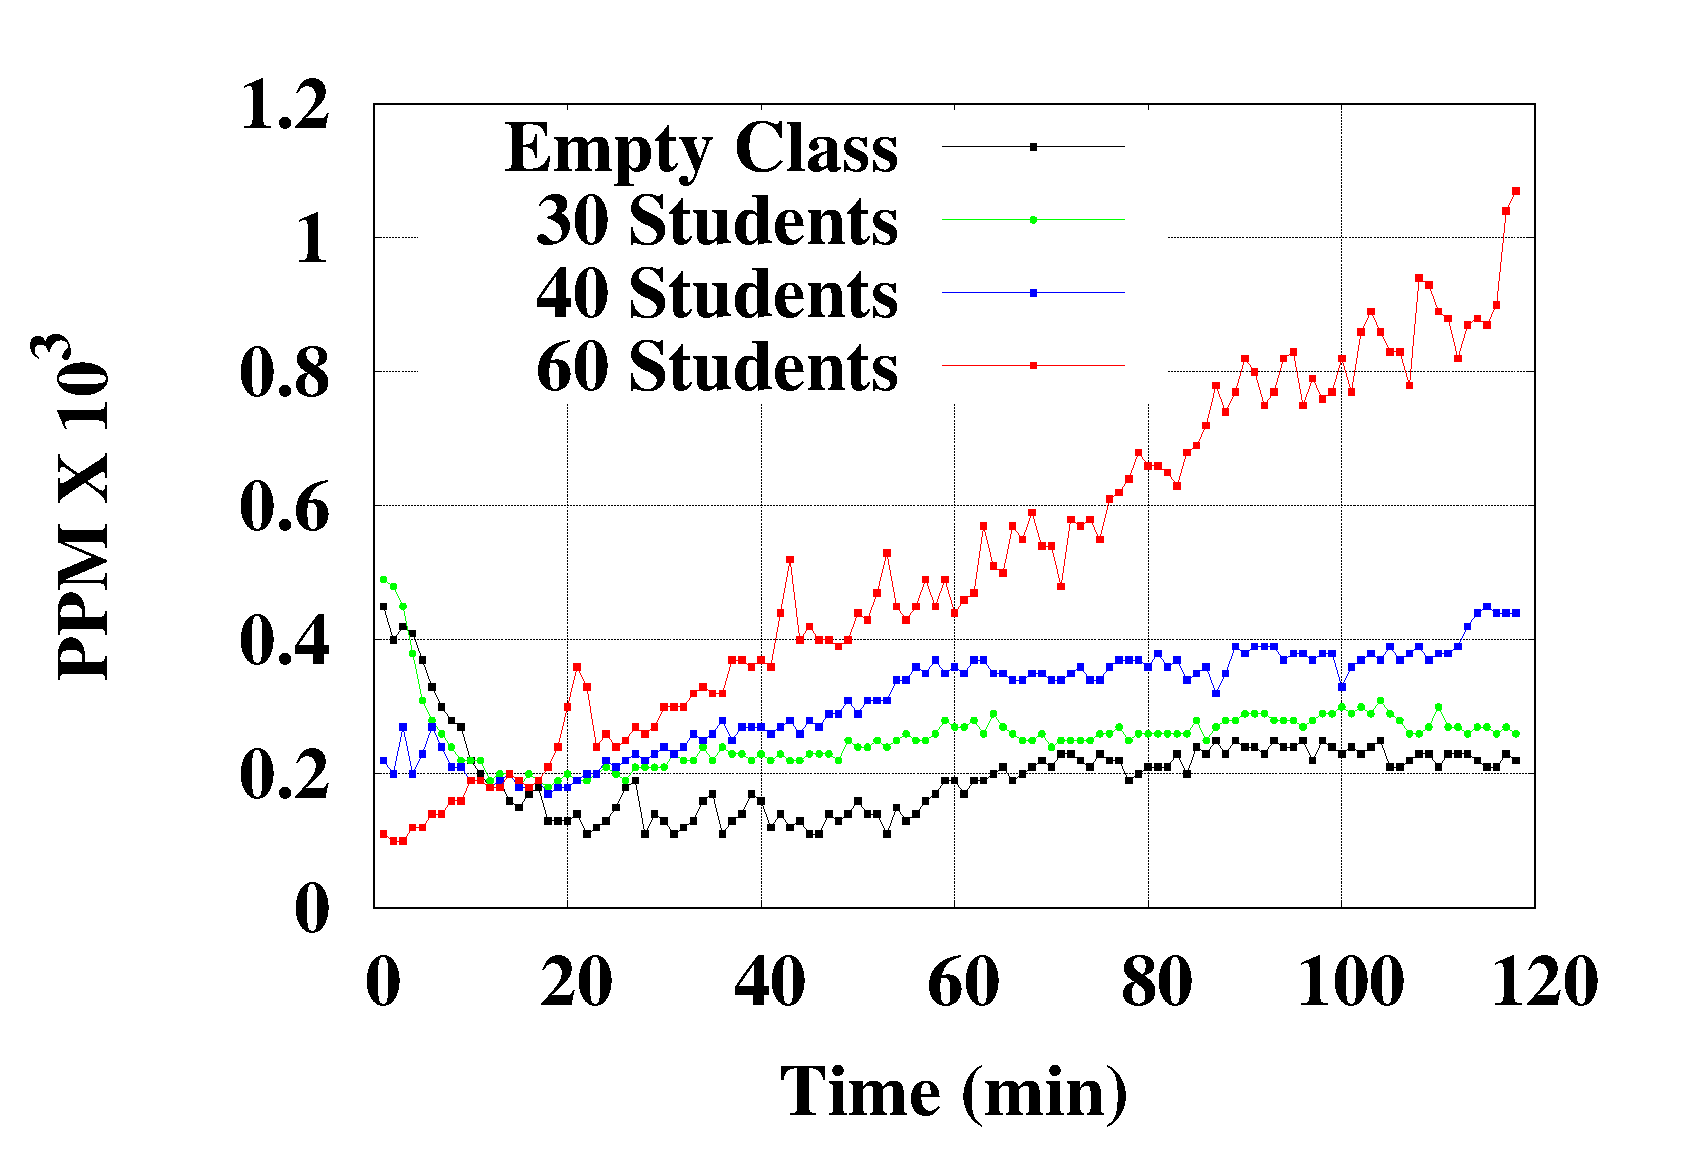
\includegraphics[height=5cm]{Final_co2.eps}}
	\hfill
	\subfigure[Impact of $PM_{2.5}$]{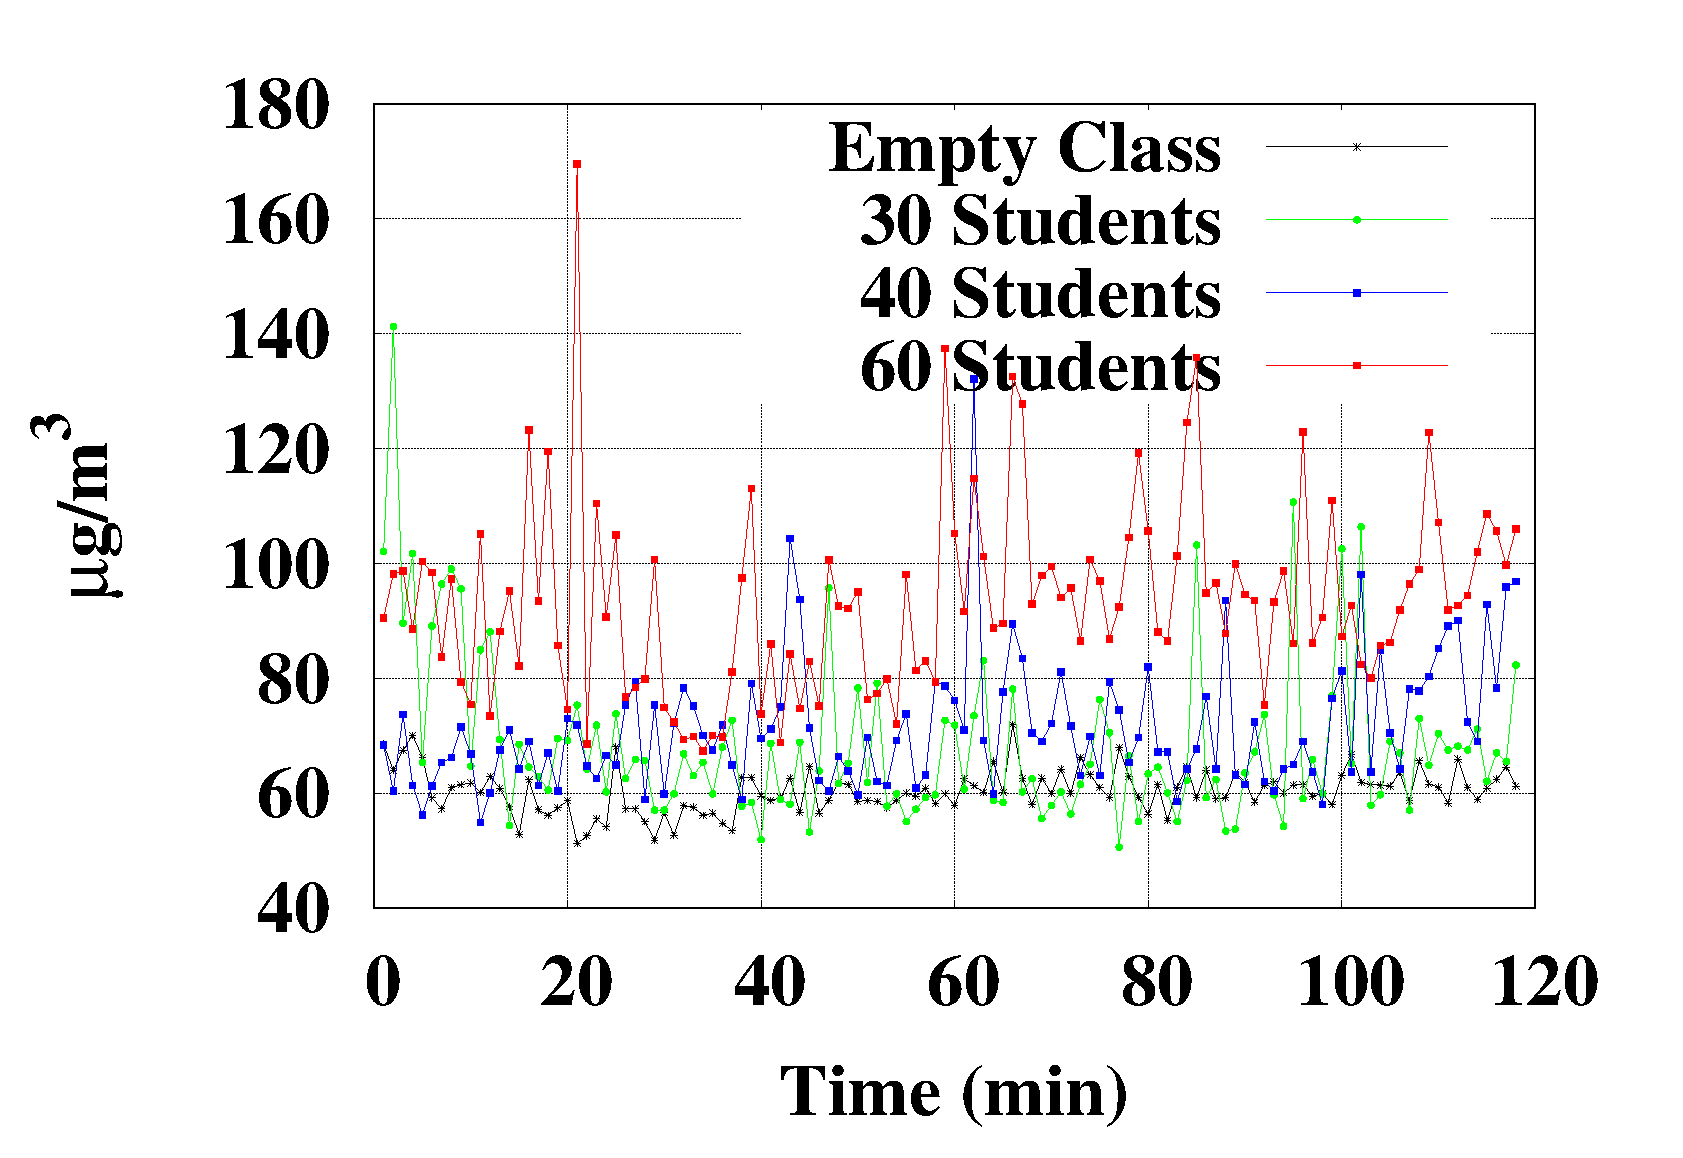
\includegraphics[height=5cm]{Final_dust.eps}}
	\hfill	
	\subfigure[Humidity label]{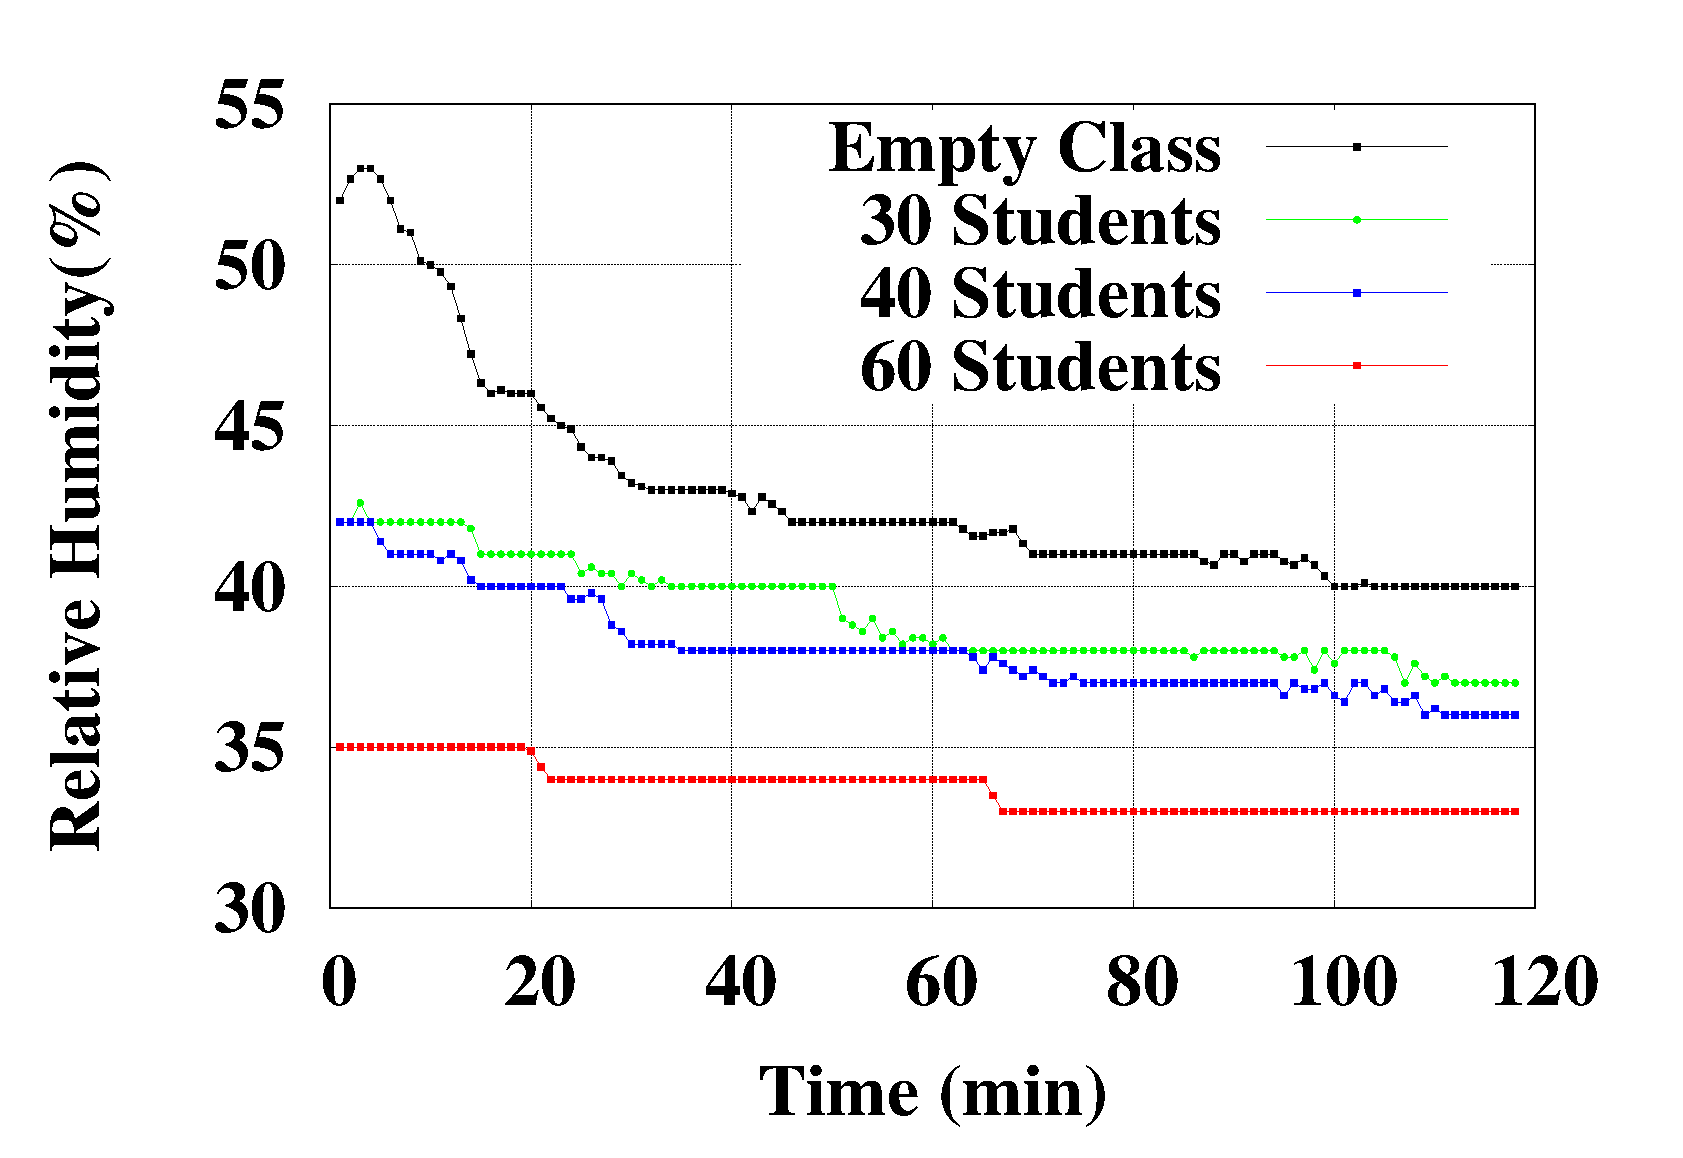
\includegraphics[height=5cm]{Final_humidity_1.eps}}
	\hfill	
	\subfigure[Temperature rise]{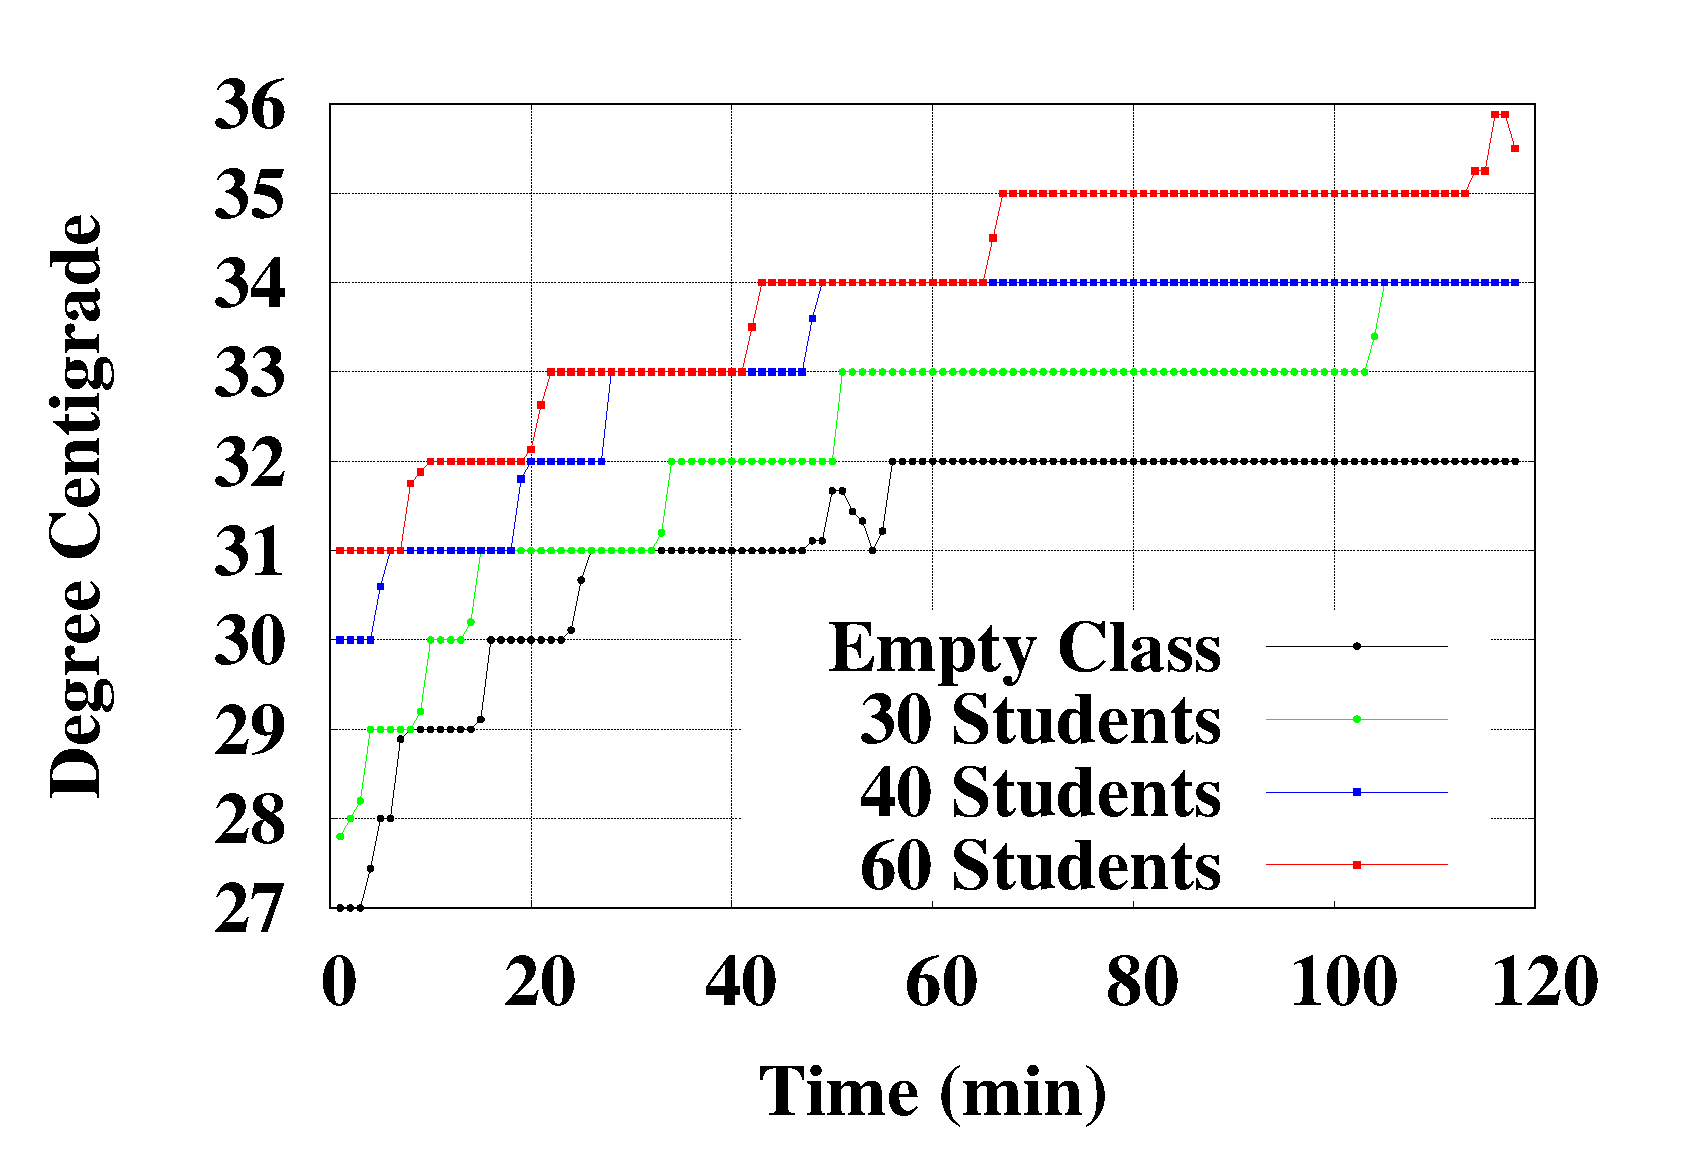
\includegraphics[height=5cm]{Final_temp.eps}}
	\hfill
	\caption{Plots showing variation of different pollution level with time.}
\end{figure}



\textbf{Impact of $CO_2$ During Class}: From the Table 2, it is clear that average $CO_2$ level for the empty classroom is 199.75 ppm which is the normal limit (ASHRAE) [8]. An adult releases appx. 12L of $CO_2$ in the duration of 1 hr class session. Hence the increase in $CO_2$ concentration is evident in the scenario with respect to student strength and existing ventilation is inadequate. In the class of 30 students $CO_2$ value rose 28.14\% with respect to the empty classroom and 55.33\% for 40 students. When there is 60 students in the room the $CO_2$ graph is increased with 173\% increase compared to empty classroom. Also from Fig. 3 for 60 students it is seen that the graph approaches 1000 ppm (ASHRAE) standard limit [8] and maximum value is 1070 ppm. Thus it can be said that it is not advisable to begin the class with 60 students. However, the class can be continued with 30 and 40 students.

\textbf{Impact of $PM_{2.5}$ During Class}: Average $PM_{2.5}$ level for the empty classroom is 60.34µg/m3 and it is varying from 51.25µg/m3 to 71.92µg/m3 which is in the normal limit (as per EPA 65µg/m3 (average)). Also in the class of 30 students the level increased to 13.25\% with respect to the empty classroom, when the strength was 40 the level of $PM_{2.5}$ increased to 21.48\% with respect to the empty classroom and the average value is 73.29µg/m3 and from the plot it is observed that after 100 minutes of class, the level steep up above 100µg/m3 which is an alarming limit that the class should be completed within 100-120 minutes of start. But with class strength 60 the $PM_{2.5}$ level is within 67.38µg/m3 and 169.57µg/m3 with a high increase of 53.77\% with respect to empty classroom. Thus the class should not be started with 60 students seeing the high value of $PM_{2.5}$ which is not advisable as per (NAAQS/EPA) standard.


\textbf{Relative Humidity and Temperature During Class}: Relative humidity(RH) and Temperature plots show an interesting characteristic, when there is increase in temperature there is fall in RH of the room. Also, for the empty classroom, the Humidity is varying from 53\% to 40\% which is within ASHRAE Standard 65\% to 30\% [9] and the temperature range is between 270C and 320C. In a class of 30 students the humidity falls by 8.88\% and temperature increased by 3.41\% with 1.060C rise with respect to empty class. Similarly, for 40 Students humidity fall by 11.38\% and there was average 2.030 rise in temperature and within 100 min of class the humidity level was 36\% which is just close the lower permissible limit which results in dryness to the students. Interestingly, for 60 Students class the humidity is within 33\% and 35\% which is very close to the lower permissible limit (30\%) with average fall of 21.46\% with respect to empty class, resulting in highly discomfort to students and decrease in their performance.



\textbf{Impact of $PM_{2.5}$ and $CO_2$ After Class}: The level of $PM_{2.5}$ is satisfactory when it ranges from 31-60 and it is moderately polluted in the range of 61-90. The level of $PM_{2.5}$ (after the class is over and the classroom is vacant) is decreasing and after 30 minutes it is dropped from 87 to 70 as shown in Fig. 4, the same effect has been noticed for $CO_2$ also. During the class hour the pollutants increase rapidly and after the class is over, the concentration of pollutants is decreasing, which can be modelled for getting the duration for which the classroom should leave vacant such that the pollutants settle down to at least satisfactory level and that classroom could be reused.
\begin{figure}
\centering
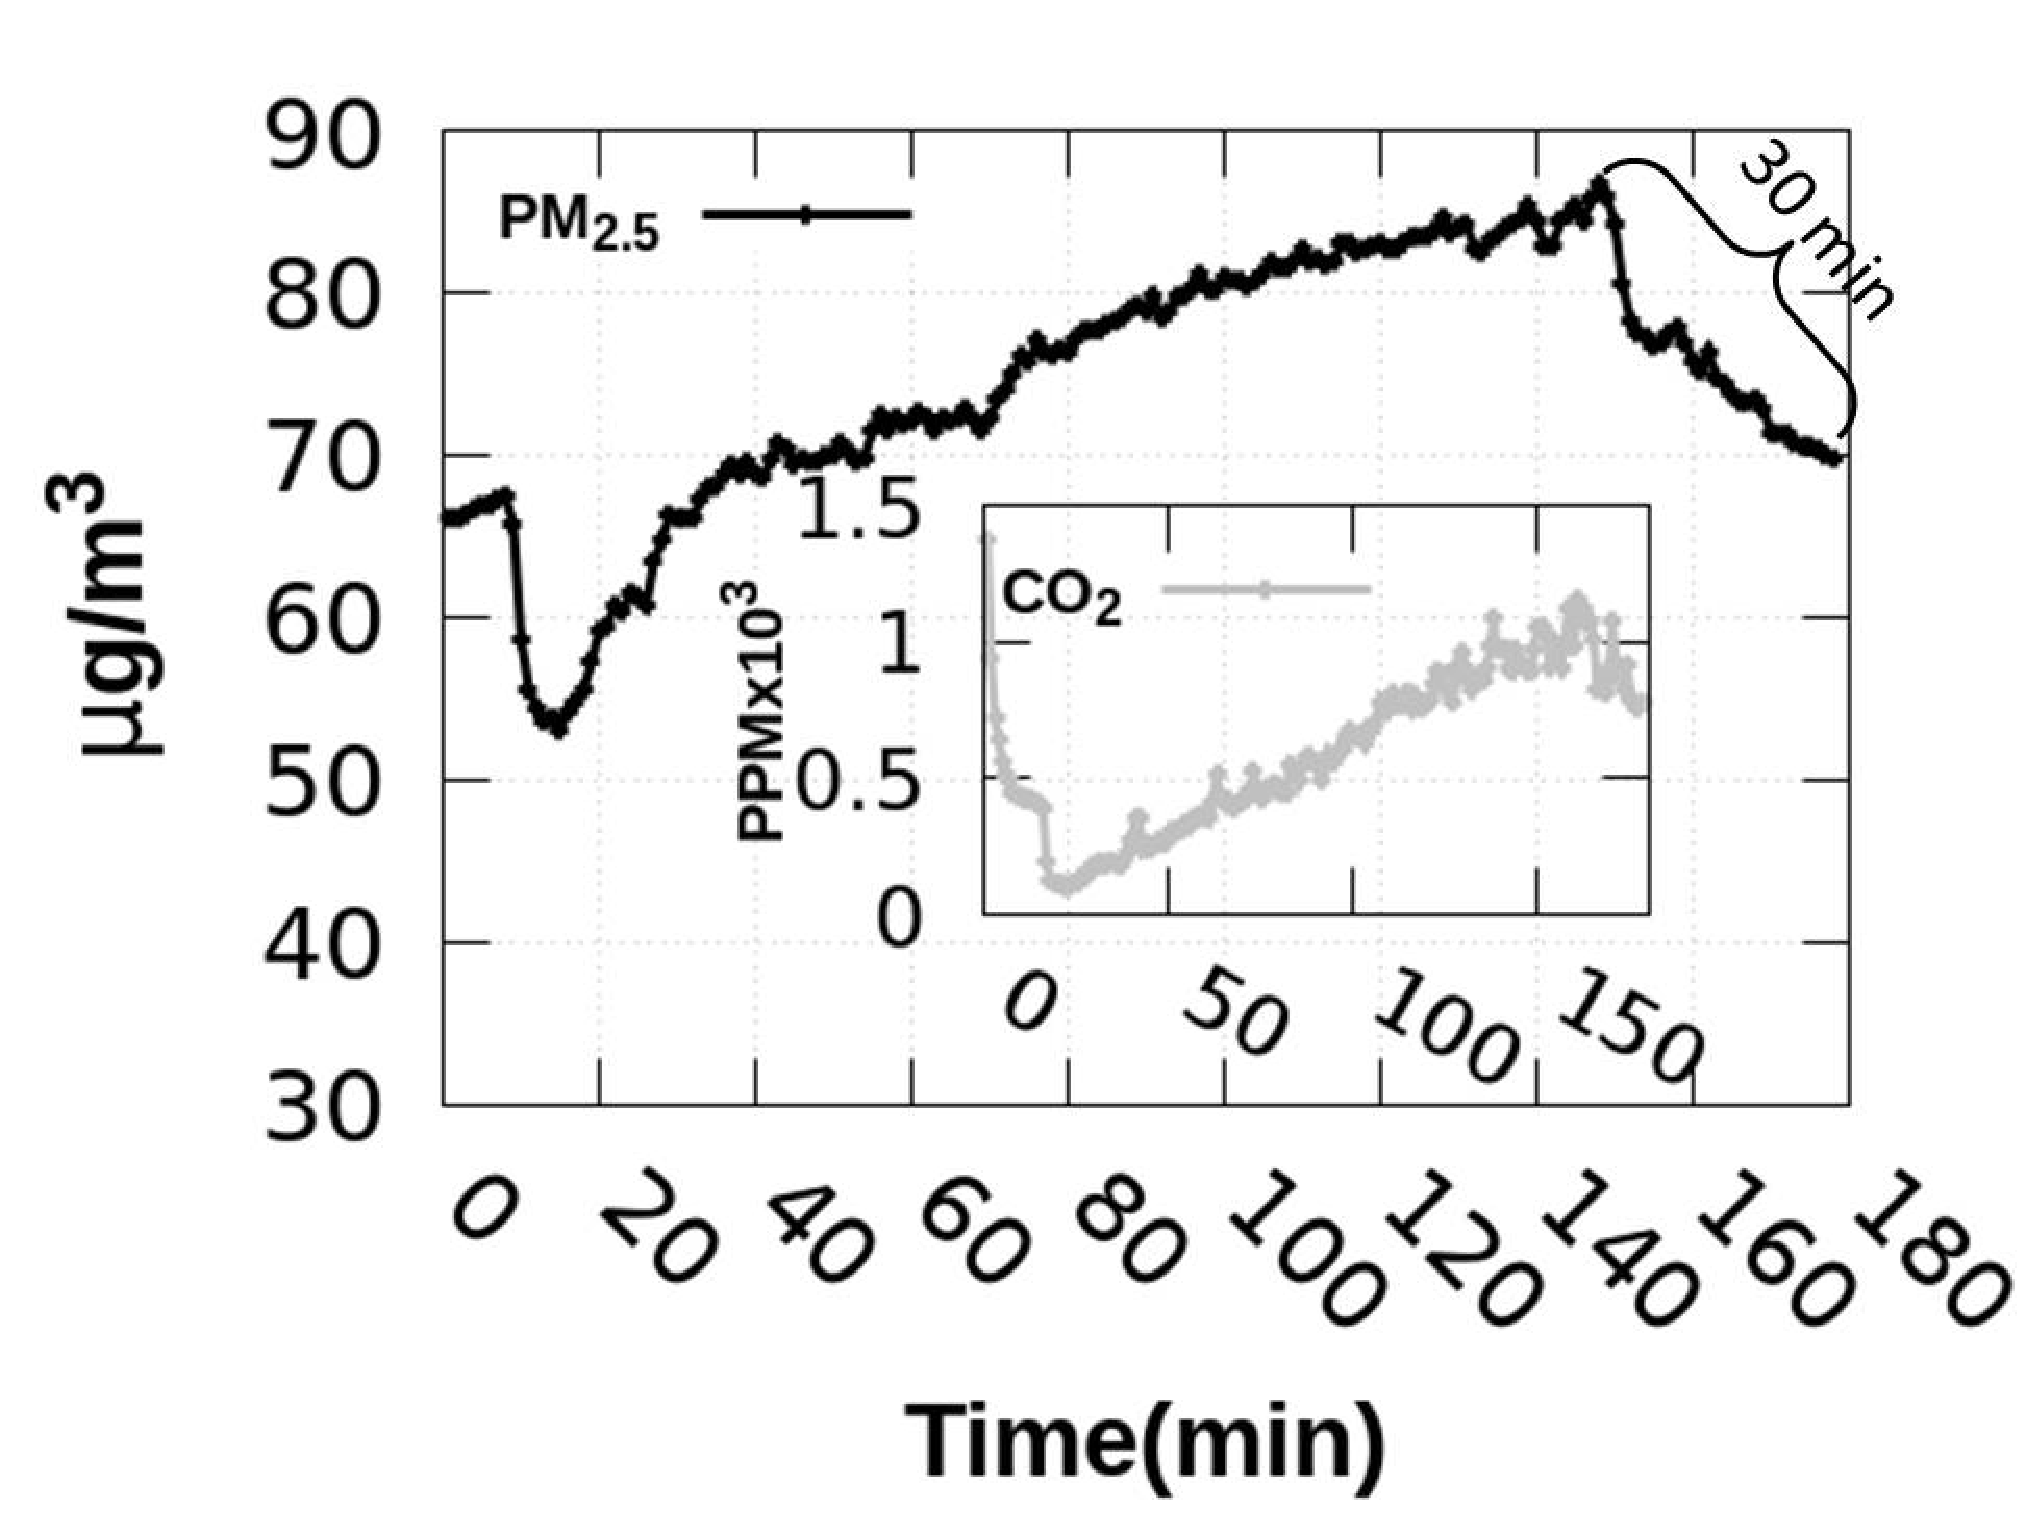
\includegraphics[width=0.5\textwidth]{./Presentation3}\\[0.1in]
\label{fig:Impact of $PM_{2.5}$ and $CO_2$}
\caption{Impact of $PM_{2.5}$ and $CO_2$}
\end{figure}

\section{Android Application}

The Android Application is having functionalities like Viewing the Current Pollutant Status, The student can have their custamized Profile and also the student can give a survey for the Environment of the Classroom.

\subsection{Current pollution status}
In this activity current concentration of the pollutant of the class is fetched from the device through server. It contains some parameter like Dust concentration, CO2 , CO , Temperature and SO2 along with current date and time of the data



\subsection{Student profile}
In this activity student can create their own profile based on their health status or prescription prescribed by doctor for some parameter like Dust Limit, CO2 gas Limit, CO gas Limit, Temperature Limit and SO2 gas limit. Current status of classroom pollution is mapped with student profile data. If any value of pollutant present currently in classroom exceeds the student profile data then application generates a notification that this environment is not fit for his/her health. He must leave the classroom as soon as possible. 

\begin{figure}
	\hfill
	\subfigure[Current Pollution Status]{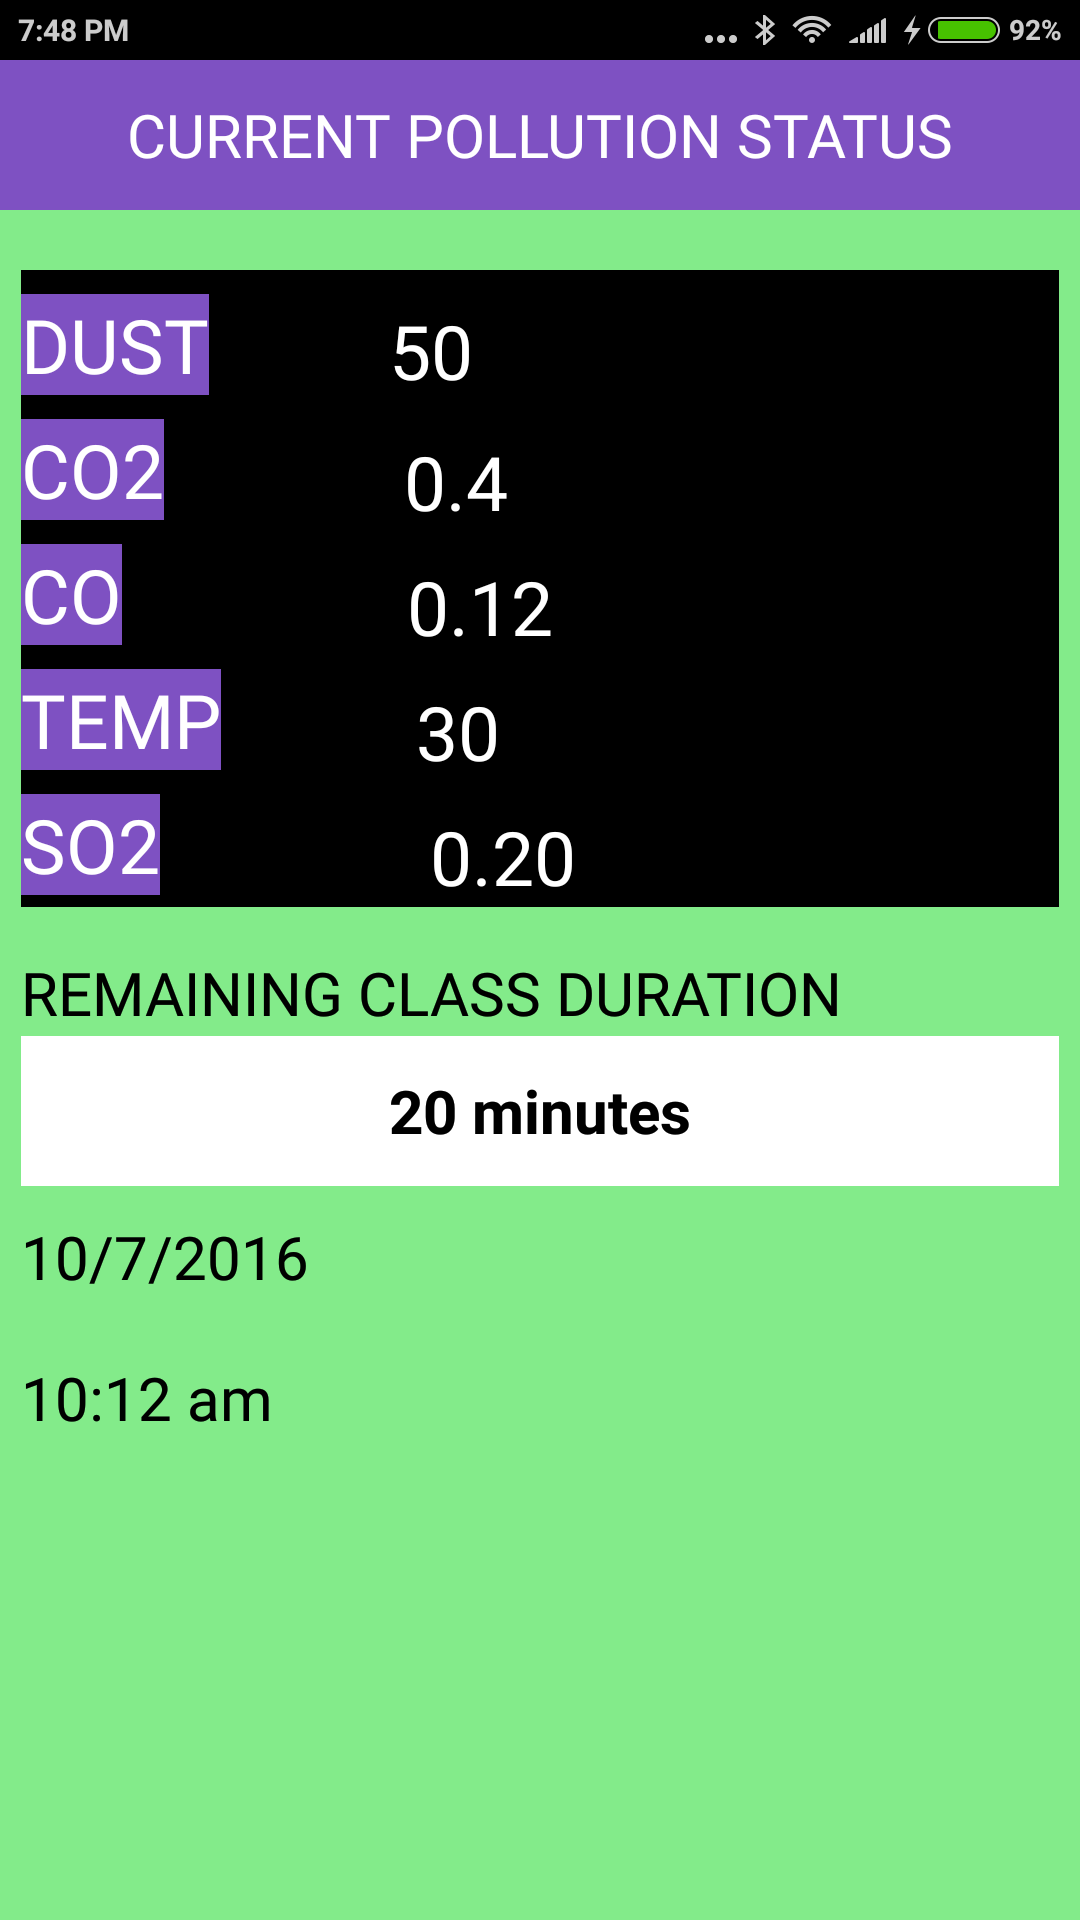
\includegraphics[width=5cm]{image3.png}}
	\hfill
	\subfigure[Student Profile]{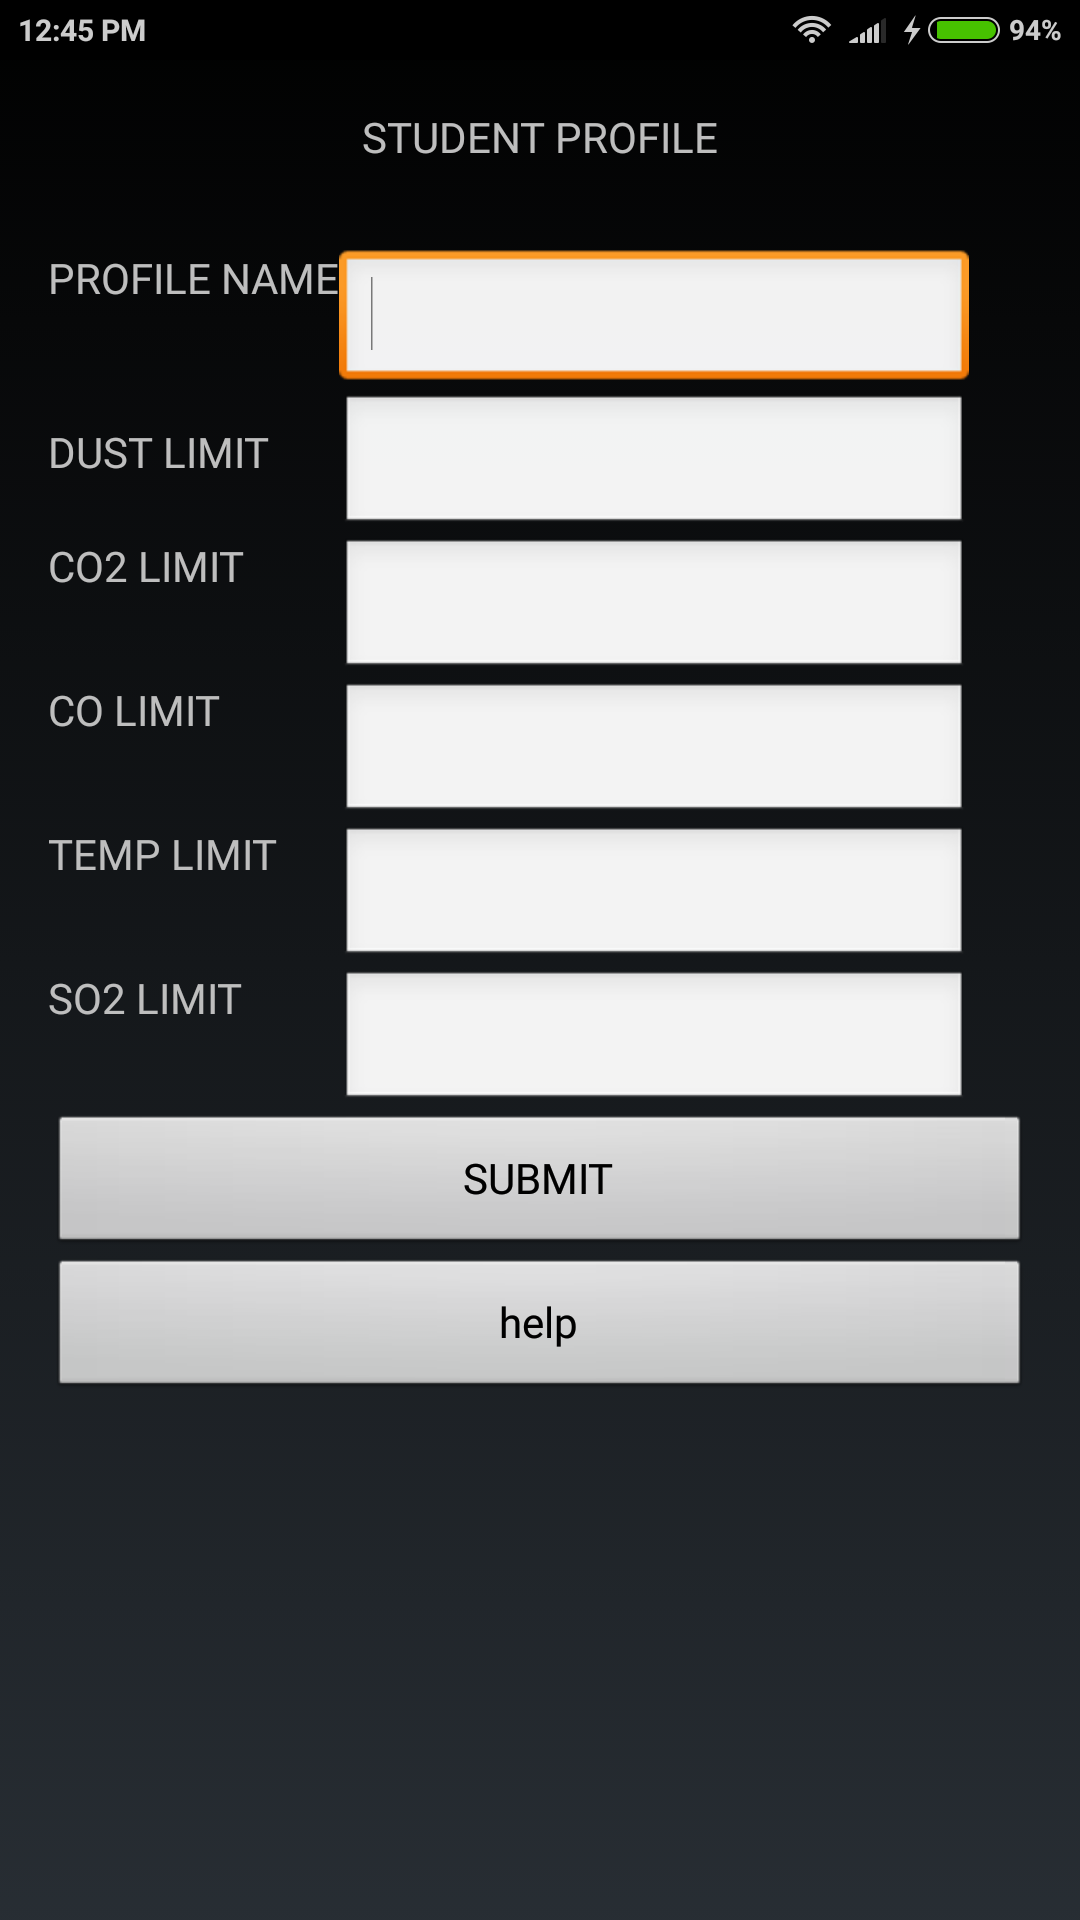
\includegraphics[width=5cm]{image4.png}}
	\hfill
	\centering
	\subfigure[Student Survey]{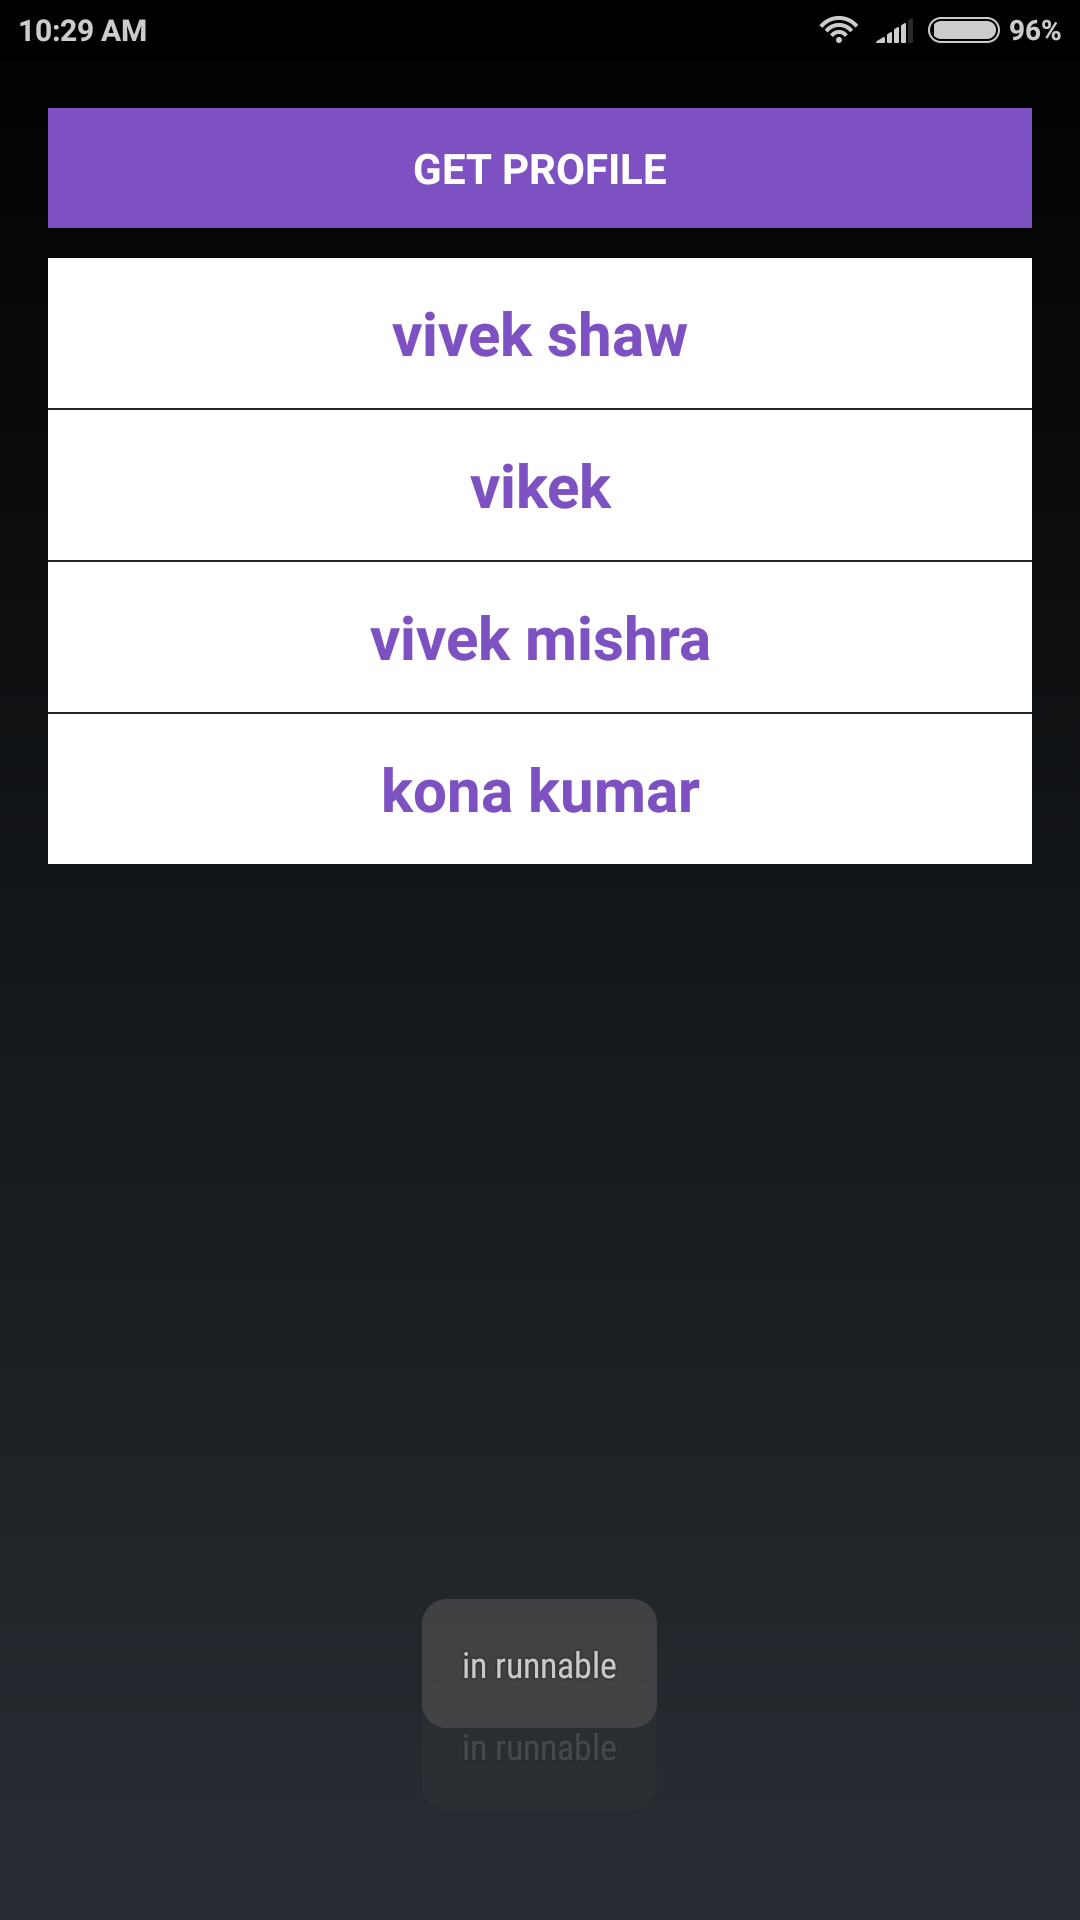
\includegraphics[width=5cm]{image5.png}}
	\hfill
	\caption{Android Application}
\end{figure}


\subsection{Student Survey}
When students are inside the classroom they can give their feedback about the overall environmental condition of the classroom. Their feedback will be saved in cloud database and administration can look into the matter for further improvement of the issue. Once students completed the feedback procedure, they will receive the confirmation mail on their registered email id.The feedback will be based on student view of the Classroom enviroment conditions.

